%%%%%%%%%%%%%%%%%%%%%%%%%%%%%%%%%%%%%%%%%%%%%%%%%%%%%%%%%%%%%%%%%%%%%%%%
%                                                                      %
%     File: Thesis_Results.tex                                         %
%     Tex Master: Thesis.tex                                           %
%                                                                      %
%     Author: Andre C. Marta                                           %
%     Last modified :  2 Jul 2015                                      %
%                                                                      %
%%%%%%%%%%%%%%%%%%%%%%%%%%%%%%%%%%%%%%%%%%%%%%%%%%%%%%%%%%%%%%%%%%%%%%%%

\chapter{Results}
\label{chapter:results}

This chapter presents the simulation results in the behaviour of the aircraft for the different solutions proposed to control and stabilise it. Once the goal for the results of this chapter is properly established, the first step will be to validate the model which has been implemented. This will be done by controlling the aircraft into cruise conditions using the baseline feedback linearisation error. The effects of disturbances and inversion errors will then be studied regarding their effects on the aircraft dynamics. Inversion errors will first be studied, first on the baseline controller then on the NN corrected controller, comparing the results of both simulations. The same methodology will then be used to study responses to system failures.

The next step will be to achieve the goal of this thesis and demonstrate the effects of an on-line neural network in reducing the tracking error in the presence of these disturbances. Finally, from the adaptive controller, including the neural network, the guiding law described in chapter \ref{chapter:implementation} in \ref{eq:guidance_law} will be added to follow a given trajectory. 
All the simulations described in this chapter were made in Matlab/Simulink with a fixed step of $f_{sample} = 30$ Hz.


%%%%%%%%%%%%%%%%%%%%%%%%%%%%%%%%%%%%%%%%%%%%%%%%%%%%%%%%%%%%%%%%%%%%%%%%
\section{Model Validation}
\label{section:results/validation}

The goal in this section will be to validate the behaviour of the model in cruise flight. Assuming cruise conditions yelds

\begin{gather}
	T=D\\
	W=L\\
	L'=M=N=0
\label{eq:cruise_cond}
\end{gather}
In order to verify the model described so far, the required thrust to have cruise conditions will be computed for a given plausible value of $\alpha$. From this point the airspeed of the aircraft can also be computed. The graph of $C_L$ versus alpha was also obtained from its respective neural network, as detailed in subsection \ref{section:model/plane_dynamics}, given by figure \ref{fig:cl_alpha}
\begin{figure}[!htb]
  \centering
  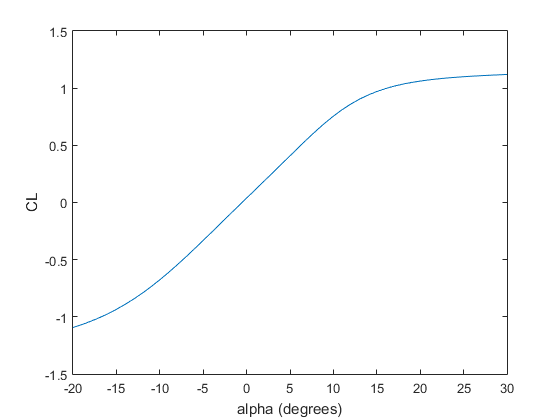
\includegraphics[width=0.75\textwidth]{Figures/CL_alpha.png}
  \caption[$C_L$ versus $\alpha$ graph]{$C_L$ versus $\alpha$ graph from Neural Network}
  \label{fig:cl_alpha}
\end{figure}
From the cruise conditions \ref{eq:cruise_cond}, knowing that $L=\dfrac{1}{2}\rho S V^2 C_L$, solving for the airspeed V comes that

\begin{equation}
V=\sqrt{\dfrac{2mg}{\rho S C_L}}
\label{eq:cruise_speed}
\end{equation}
The required thrust can also be computed from \ref{eq:cruise_cond}, \ref{eq:cruise_speed}, \ref{eq:forces} and \ref{eq:cd_cl}, knowing $C_L$ for a given angle of attack. Proposing some values of $\alpha$, the following results are obtained

\begin{table}[htbp]
  \centering
  \caption{Required cruise conditions for different values of $\alpha$}
    \begin{tabular}{ccccc}
    \toprule
    $\alpha (^o)$ & $C_D$ & $C_L$ & $V (ms^{-1})$ & $T (N)$ \\
    \midrule
    0     & 0.017677131 & 0.0387 & 707.4010791 & 224047.3585 \\
    2     & 0.019379779 & 0.1859 & 322.7613368 & 51133.84325 \\
    4     & 0.023345134 & 0.334 & 240.7952785 & 34283.79709 \\
    6     & 0.029604436 & 0.4828 & 200.279994 & 30076.58604 \\
    \bottomrule

    \end{tabular}
  \label{tab:cruise_cond}%
\end{table}%

From these values, to test both the model (as well as the methods used to simulate the dynamics of the aircraft, including the coefficients neural networks) and the feedback linearisation controller, the following references $V_a^d=200 ms^{-1}$, $\gamma^d = 0\text{ rad}$ and $\psi^d=0\text{ rad}$ were used in an attempt to simulate cruise conditions. From there, the values of thrust and angle of attack were computed and  compared to the theoretical values of table \ref{tab:cruise_cond}.
 
Following these constant reference values the results obtained can be seen in figure \ref{fig:model_validation}.

\begin{figure}
\centering
\begin{minipage}{\textwidth}
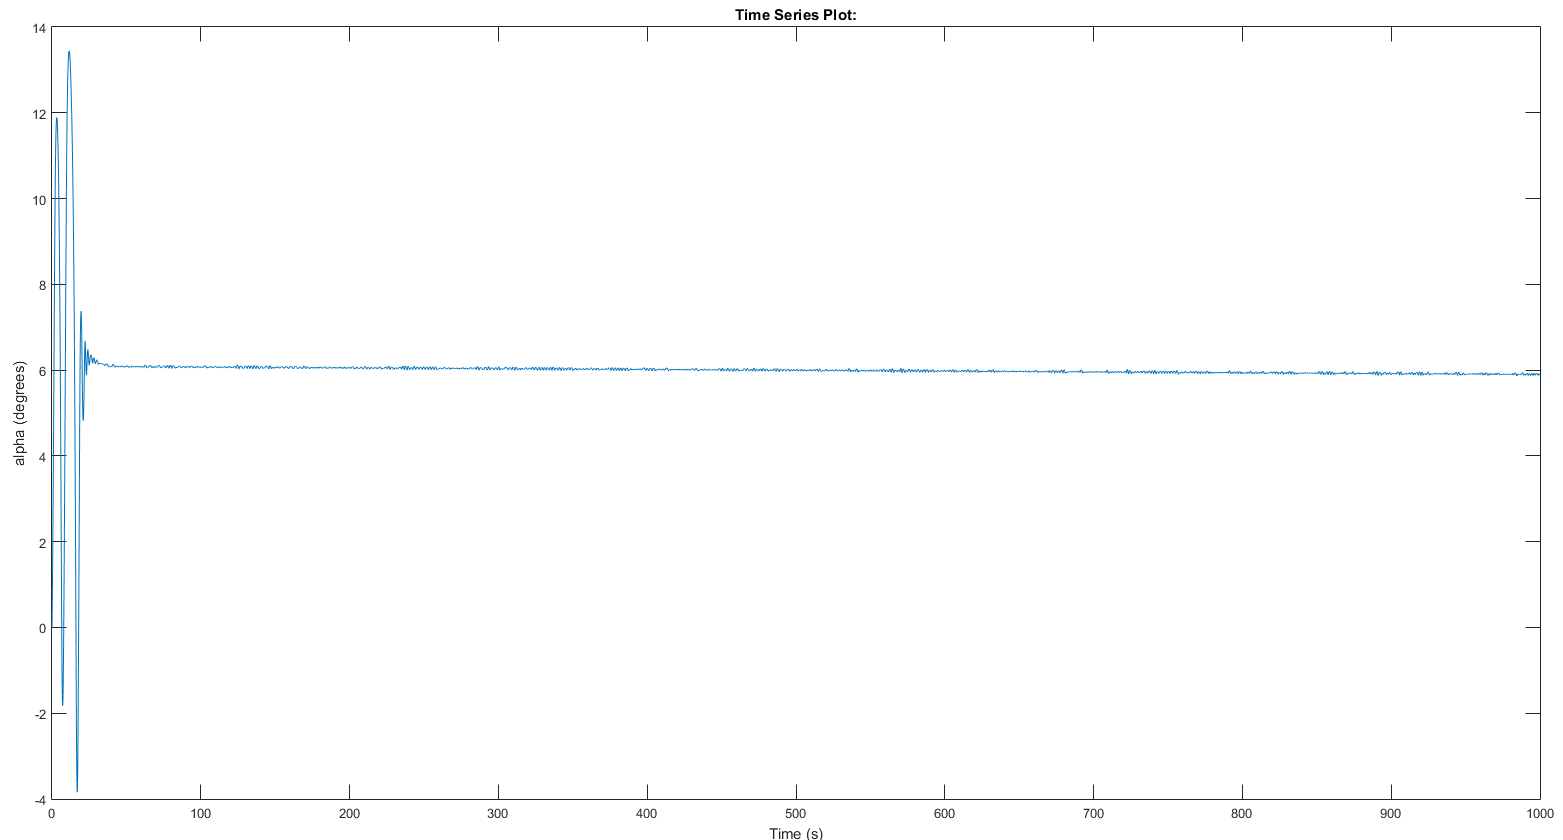
\includegraphics[width=1.1\textwidth]{Figures/Results/aoa_check.PNG}
\end{minipage}
\begin{minipage}{\textwidth}
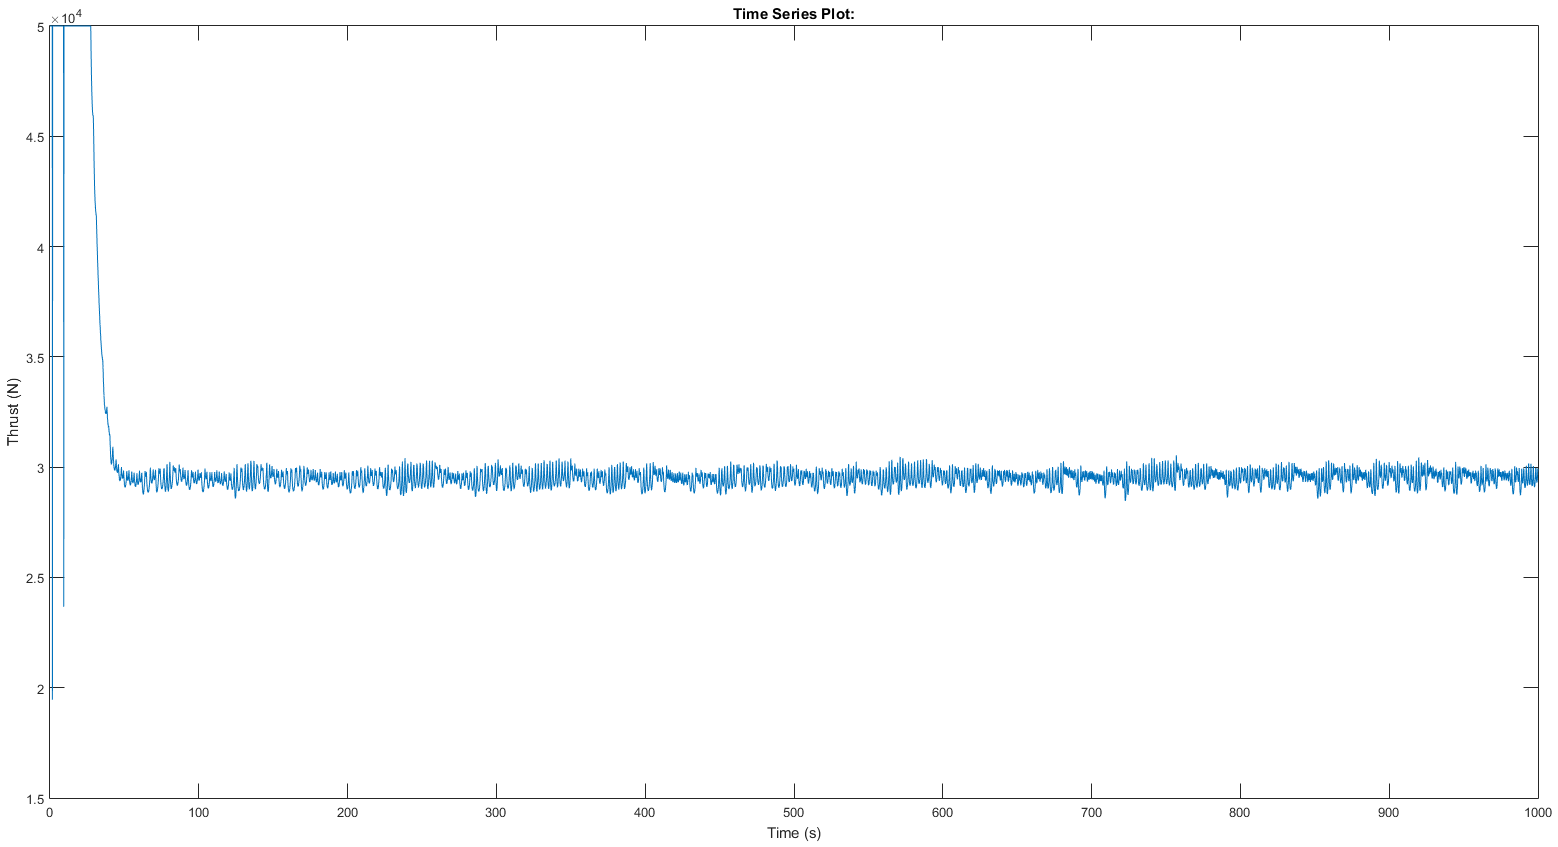
\includegraphics[width=1.1\textwidth]{Figures/Results/thrust_check.PNG}
\end{minipage}
\caption[AoA and thrust validation]{Angle of Attack (degrees) and thrust (N) of the controlled aircraft as described in the block diagram \ref{fig:controller_noNN}}
\label{fig:model_validation}
\end{figure}

This simulation, made over 800 seconds, shows clearly that the angle oscillates around a $6^o$ degree angle of attack. As for thrust, it also oscillates around $30000N$. These values correspond to the theoretical values in table \ref{tab:cruise_cond} for $\alpha=6^o$, indicating that not only the modelled plane is well behaved, but also that the NN coefficients are able to simulate an accurate model of the aerodynamic coefficients variation. Notice however that the thrust reaches its saturation value of $50\text{ kN}$ before stabilizing.
%%%%%%%%%%%%%%%%%%%%%%%%%%%%%%%%%%%%%%%%%%%%%%%%%%%%%%%%%%%%%%%%%%%%%%%%
\section{Feedback Linearisation Controller}
\label{section:results/fl_contro}

Once the model has been tested and validated, the described nonlinear inversion controller can be tested. Reference tracking will first be observed with simple constant reference values, without any guidance control law. 

Reiterating the example from the previous section, the reference following for $V_a^d=200 ms^{-1}$, $\gamma^d = 0\text{ rad}$ and $\psi^d = 0\text{ rad}$ can be seen in figure \ref{fig:const_ref}.
\begin{figure}[h]
\centering
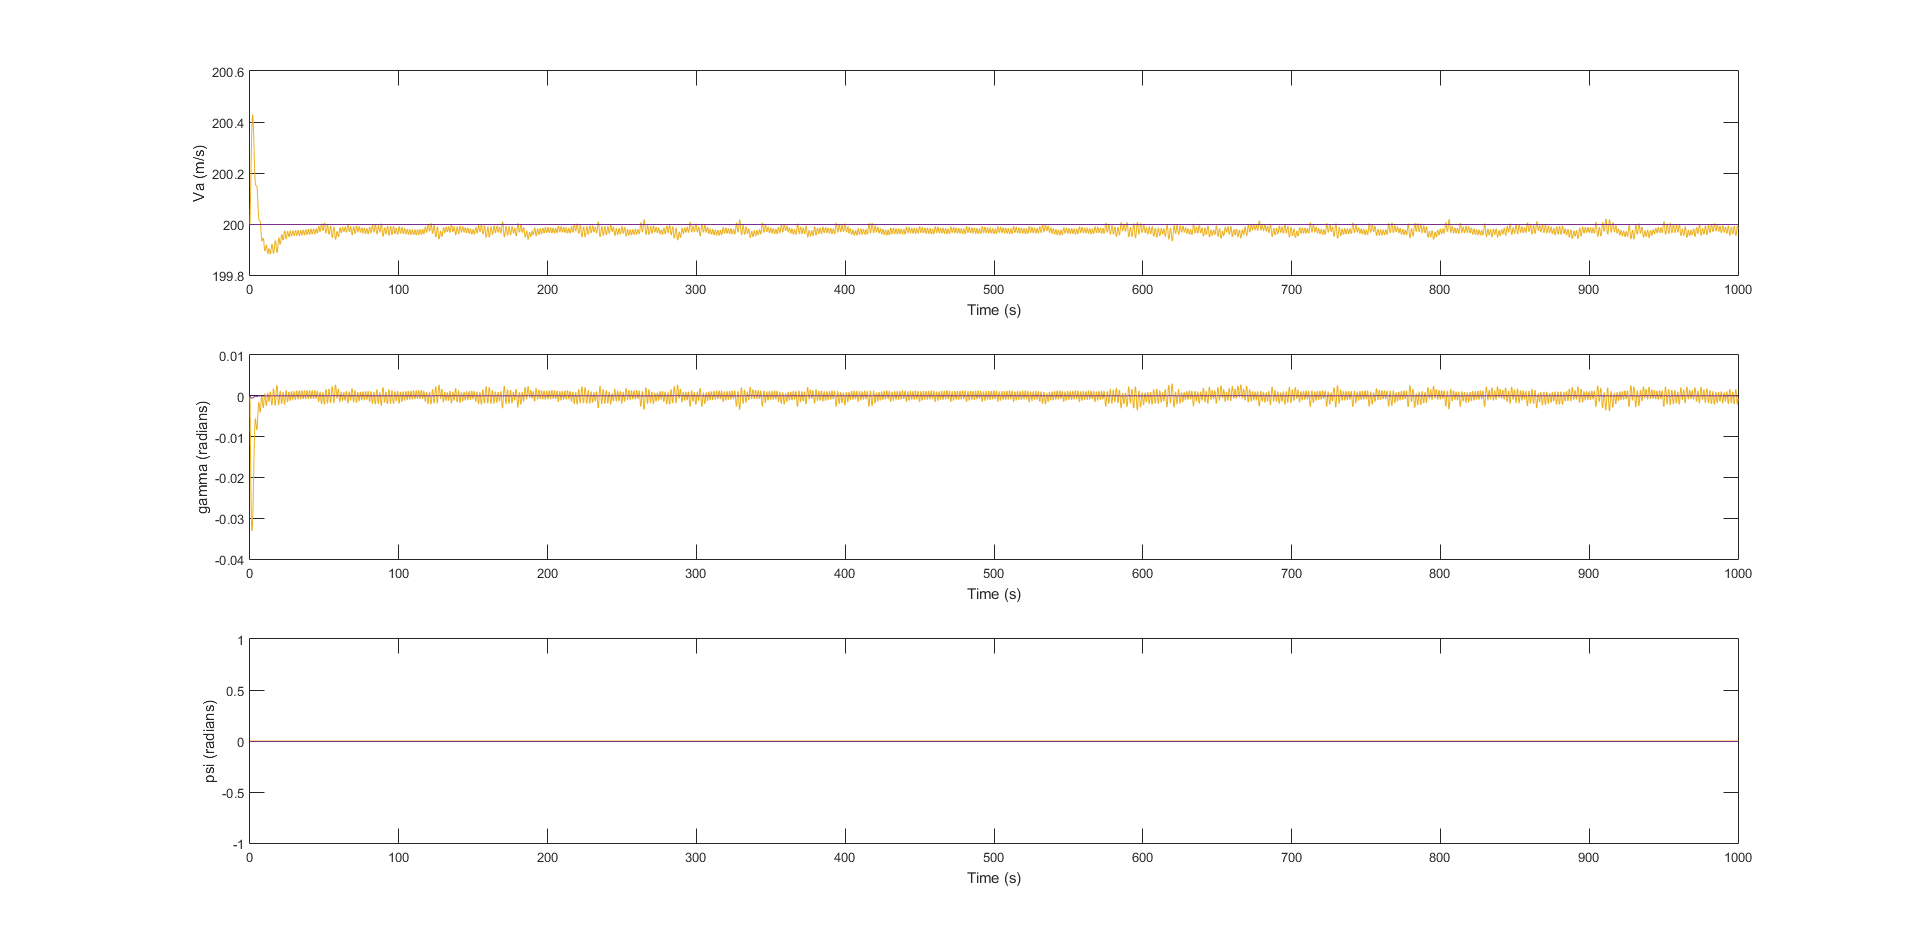
\includegraphics[width=1.1\textwidth]{Figures/Results/nli_test_const.png}
\caption[Constant heading reference following of feedback linearisation controller]{Reference (blue) following over $1000s$ of simulation time for $V_a^d=200 ms^{-1}$, $\psi^d = 0\text{ rad}$ and $\gamma^d = 0\text{ rad}$ respectively and measured values (yellow)}
\label{fig:const_ref}
\end{figure}

In figure \ref{fig:const_ref} the reference is followed with small osculations for the three variables, although with the presence of some steady state error in the case of the airspeed $V_a$. The small initial convergence of $\gamma^d$ and $V_a^d$ can be explained by the simulation initial conditions. To maintain $V_a^d=200ms^{-1}$ at $t=0s$, as seen in table \ref{tab:cruise_cond}, the AoA must be $\alpha=6^o$. As this simulation starts in cruise condition with the initial condition $\theta=0 \text{ rad}$, for this reason $\gamma$ initially takes negative values before reaching and stabilizing at its desired reference. This also affects the airspeed of the aircraft, although only increasing the following error up to $0.4ms^{-1}$.

To be able to follow trajectories however, a good control of the aircraft heading will be necessary. Proposing this time the following variation in $\psi^d$ as a reference for the simulated aircraft
\begin{equation}
\psi^d = \begin{cases}
0\text{ rad} & t < 100\\
\dfrac{\pi}{2}\text{ rad} & 100 \leq t < 500\\
0\text{ rad} & t > 500 \\
\end{cases}
\label{eq:test_traj}
\end{equation}
The comparison of the measured heading $\psi$ and its desired value comes in figure \ref{fig:heading_test}.
\begin{figure}[H]
\centering
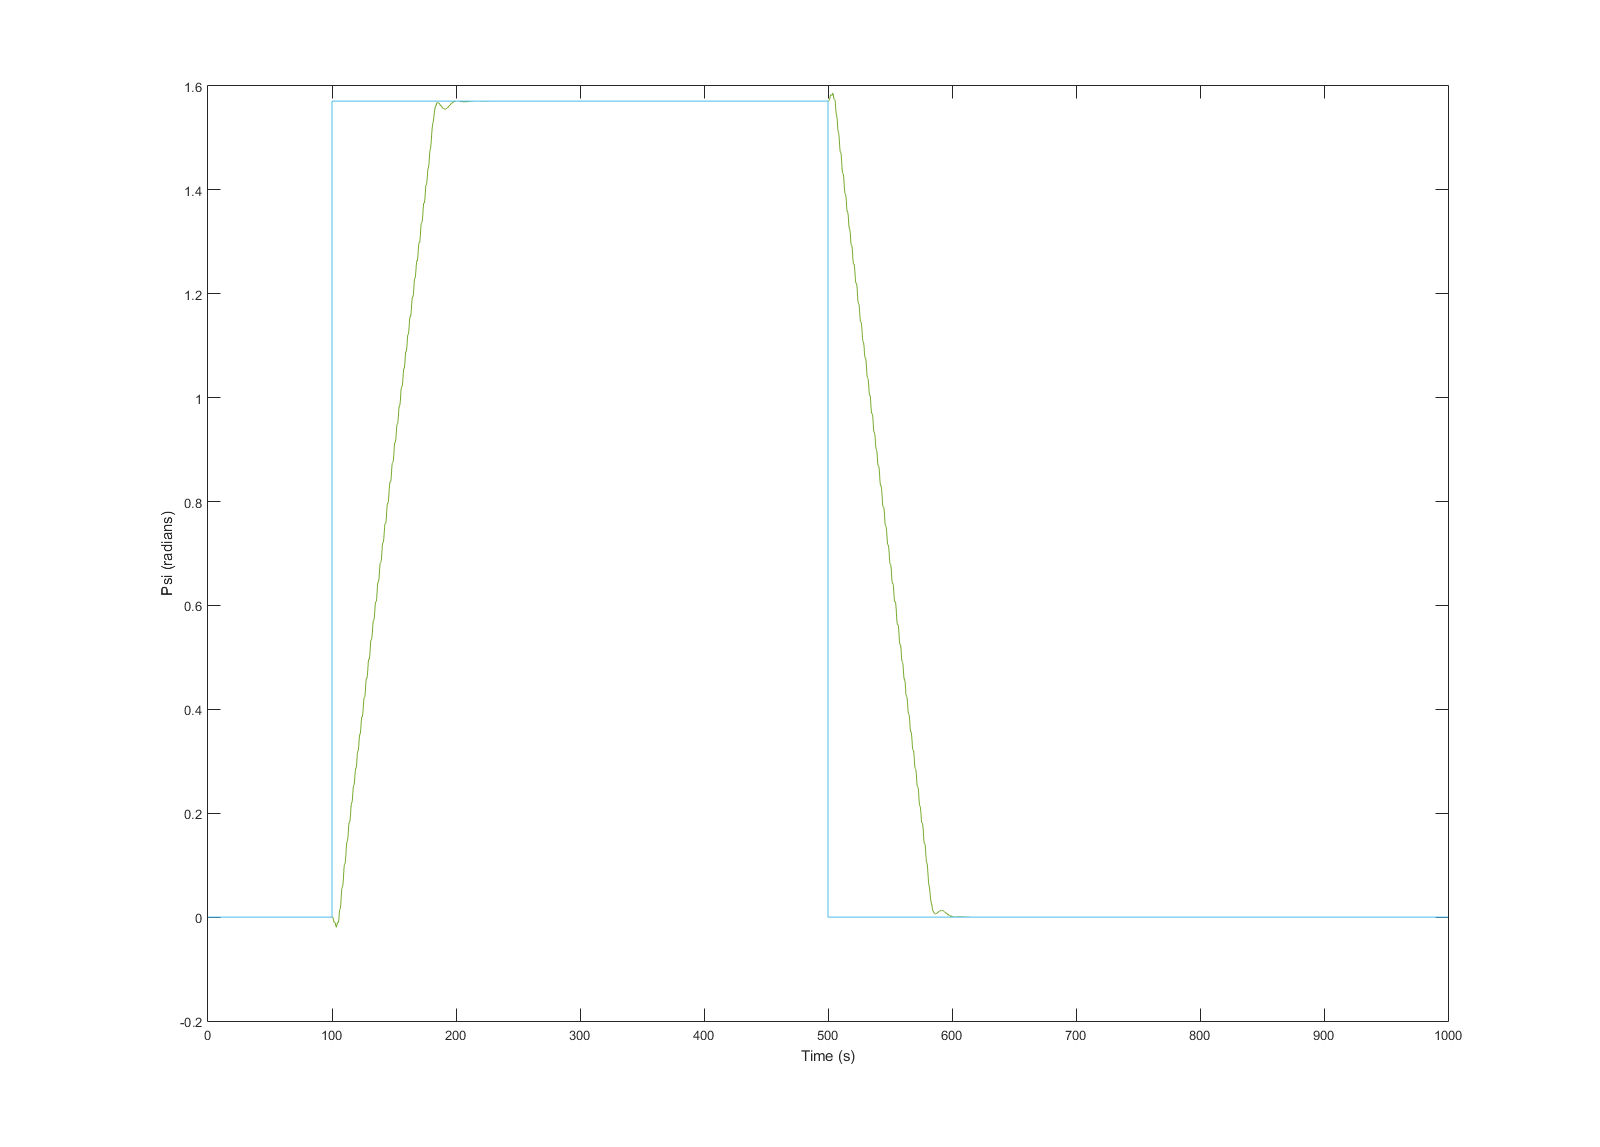
\includegraphics[width=\textwidth]{Figures/Results/heading_test.png}
\caption[Desired and measured heading]{Desired (blue) and measured (green) heading}
\label{fig:heading_test}
\end{figure}

Although the reference value is reached after each step, the convergence takes around $100s$ for a $\dfrac{\pi}{2}\text{ rad}$ perturbation to converge, without overshoot. These conversion times can be explained by the high inertia and mass of the commercial aircraft. The resulting airplane trajectory can be seen in figure \ref{fig:trajectory}.

\begin{figure}[H]
\centering
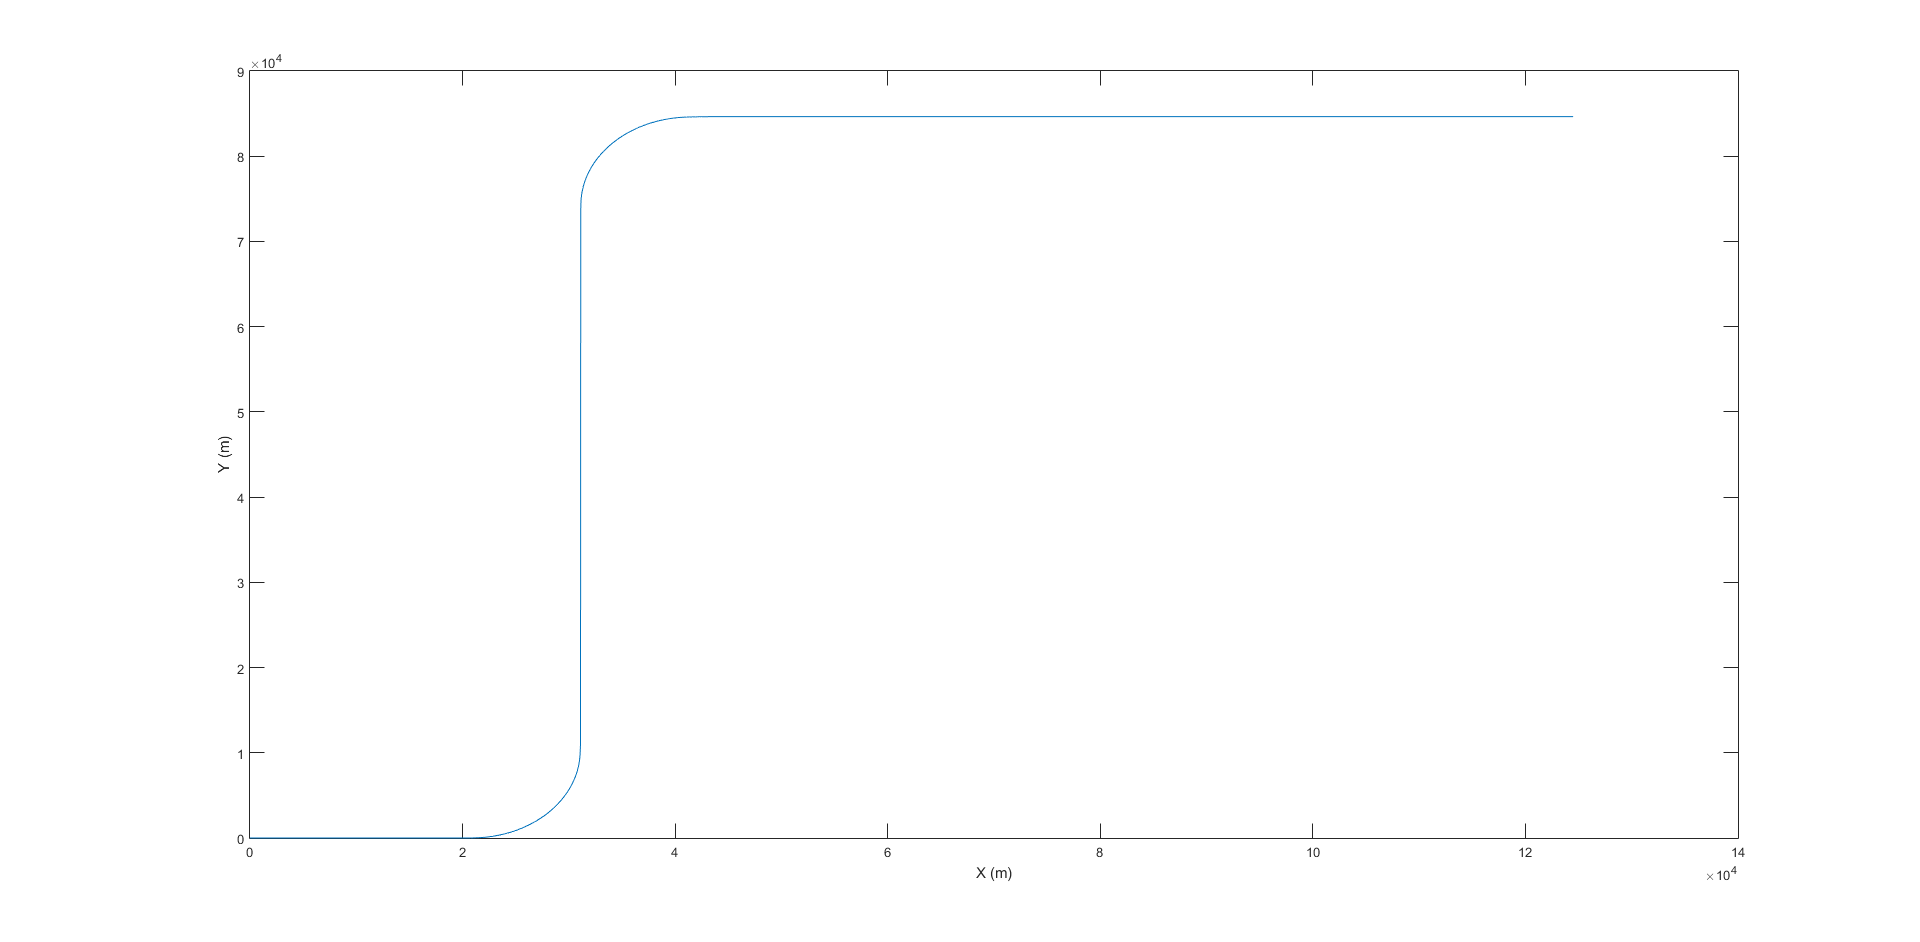
\includegraphics[width=\textwidth]{Figures/Results/trajectory.png}
\caption[Plane trajectory]{Plane trajectory for the nominal control input $\zeta=1$}
\label{fig:trajectory}
\end{figure}

From the results obtained so far, it can be concluded that the controller performs correctly following the desired reference. These results however were obtained assuming that the exact model of the aircraft was known, without any kind of external perturbation or simulated system failure. It is these perturbations that will be simulated in this section and studied. To do so the same testing reference as described in equation \ref{eq:test_traj} will be used to compare the effects of different types of disturbances with the undisturbed system.

\begin{figure}[H]
\centering
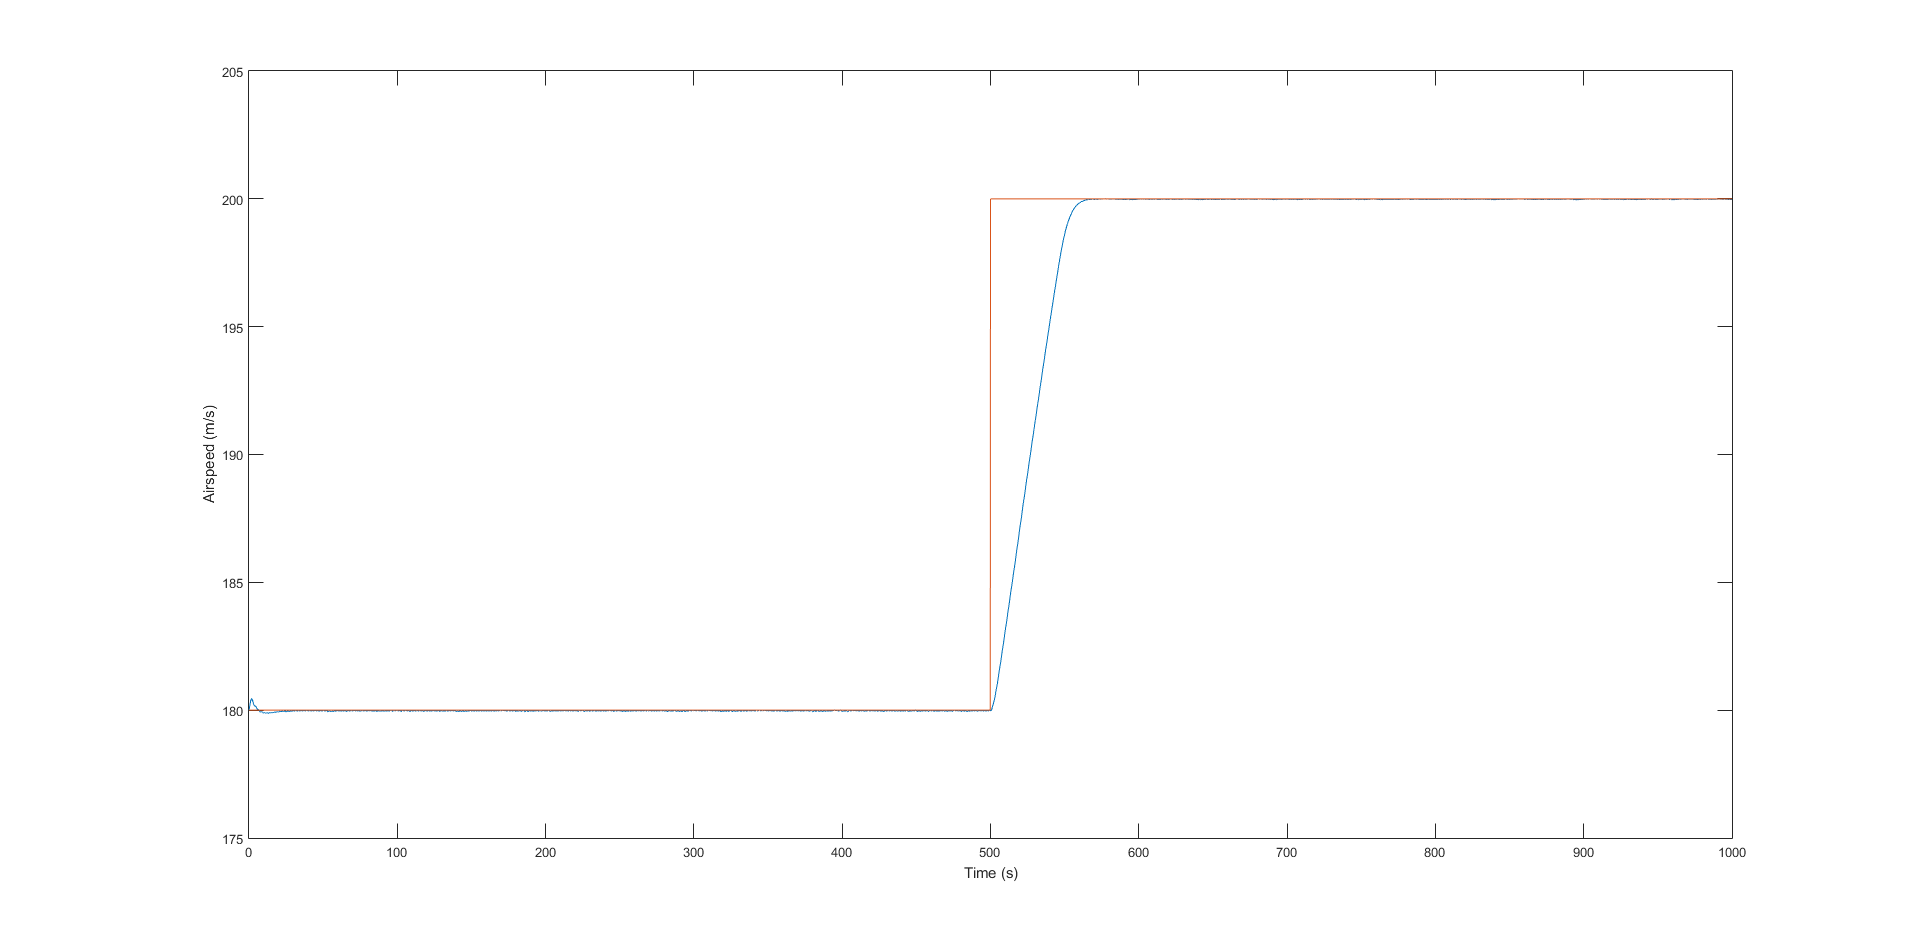
\includegraphics[width=1.1\textwidth]{Figures/Results/speed_command.png}
\caption[Airspeed reference following]{Desired (orange) and measured (blue) airspeed}
\label{fig:speed_command}
\end{figure}

In figure \ref{fig:speed_command} a step input was given as an airspeed command, going from $180ms^{-1}$ to $200ms^{-1}$. As can be observed after a delay of approximately $60s$ the aircraft reaches and stabilizes at the new airspeed reference.
\section{Inversion Errors}
\label{section:results/inversion_errors}
	
\subsection{Baseline Feedback Linearisation Controller}
This error will be the most frequent when implementing such a controller, as some system parameters estimations may have considerable errors, namely the aircraft inertial matrix. Fortunately, the controller used is, as it will be demonstrated, tolerant to errors in the estimation of this parameter, but can result in an unstable system in extreme cases. To simulate estimation errors, the entries of the inertial matrix $I_{xx}$,$I_{yy}$,$I_{zz}$ and $I_{xz}$ were multiplied by a reducing factor $\zeta \in [0;1]$ when computing the nonlinear inversion in \ref{eq:control_law}. The inertial matrix used in this equation $I_{est}$ is therefore given by $I_{est} = \zeta I$.

Changing the values of $\zeta$ to $0.5$ and $0.05$, increasing the inversion error, results in the following trajectories in figure \ref{fig:inversion_error}

\begin{figure}[H]
\centering
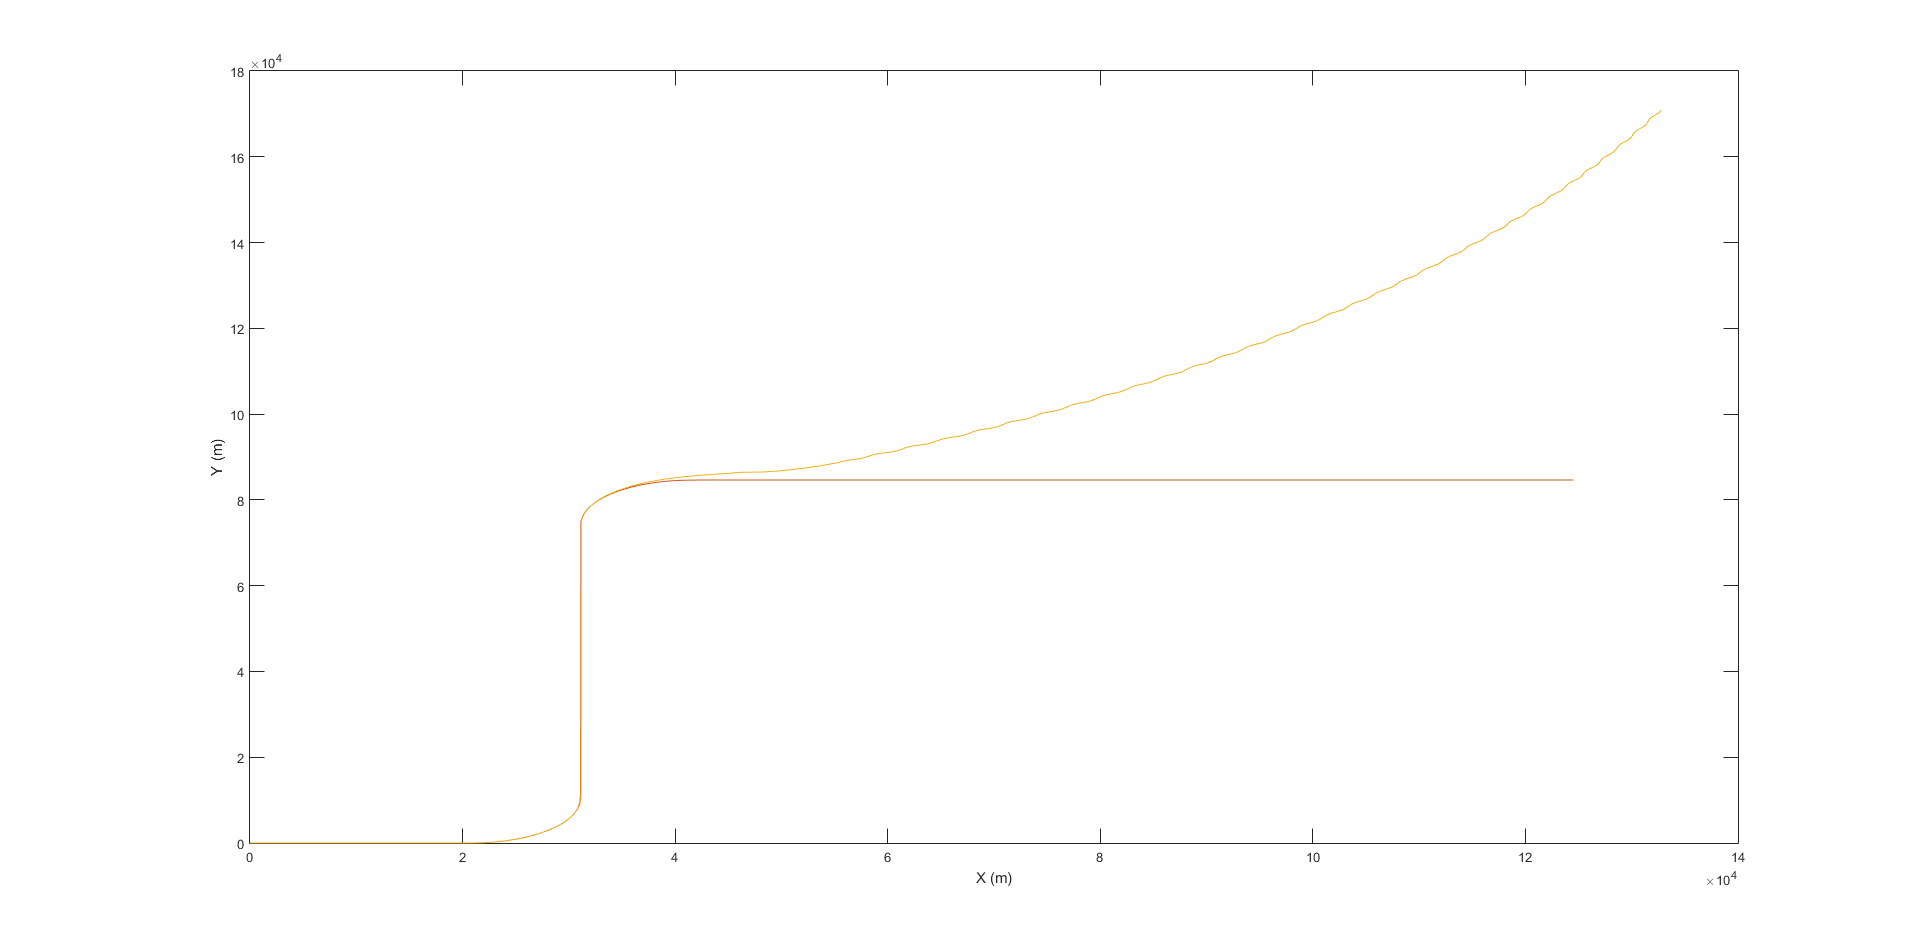
\includegraphics[width=\textwidth]{Figures/Results/inversion_error.png}
\caption[Plane trajectory with inertia estimation errors]{Plane trajectory for $\zeta = 0.5$ (red) and $\zeta= 0.05$ (yellow)}
\label{fig:inversion_error}
\end{figure}

Indeed, a 50\% error in estimating the inertia of the aircraft when computing the feedback linearisation law results in a negligible reference tracking error, as can be seen in figure \ref{fig:ref_zeta_05}. This however is not the case if $\zeta$ is reduced even further to $\zeta = 0.05$ and if the error of the system relative to its references becomes much greater (figure \ref{fig:ref_zeta_005}). As can be seen in figure \ref{fig:inversion_error}, the aircraft is unable to follow yaw demands in this case as it goes unstable. This establishes a first goal to measure the performance of the designed neural network, to try reduce the error for $\zeta = 0.05$, ultimately achieving the performance of a nonlinear inversion with no inertia estimation errors.

\begin{figure}[H]
\centering
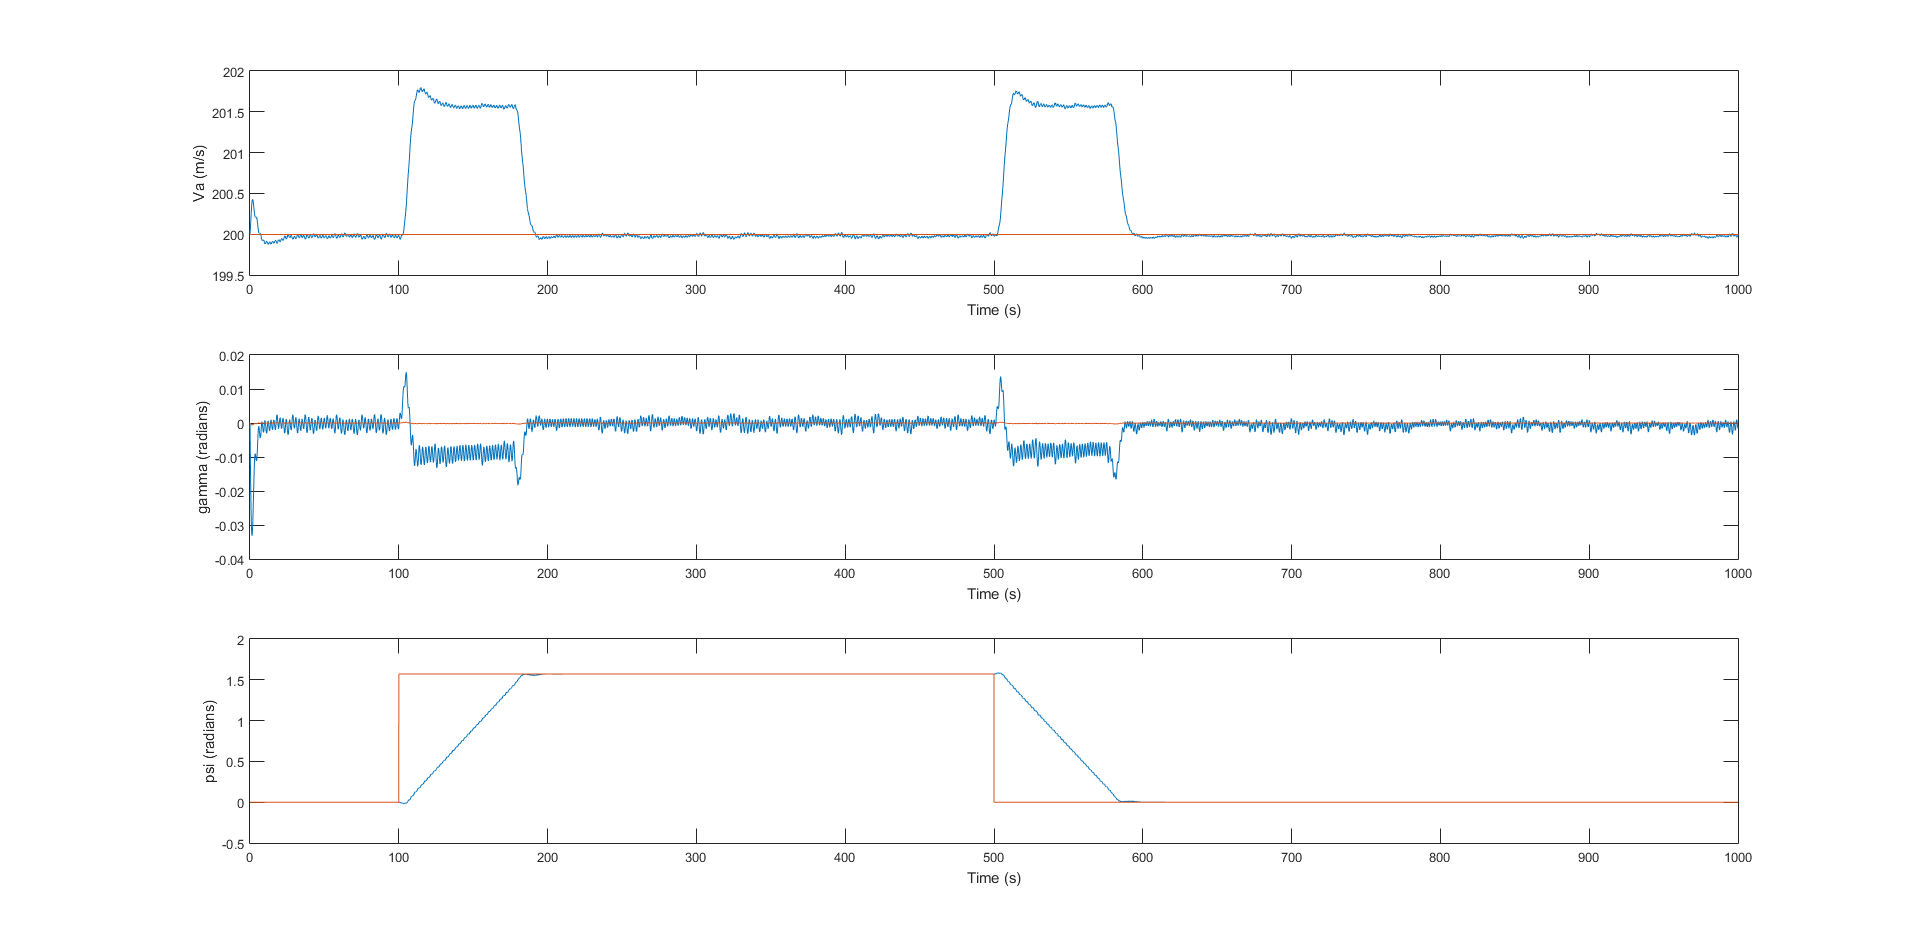
\includegraphics[width=1.1\textwidth]{Figures/Results/ref_zeta_05.png}
\caption[Reference tracking for $\zeta=0.5$]{$V_a$, $\gamma$ and $\psi$ for measured and desired values for $\zeta=0.5$}
\label{fig:ref_zeta_05}
\end{figure}
\begin{figure}[H]
\centering
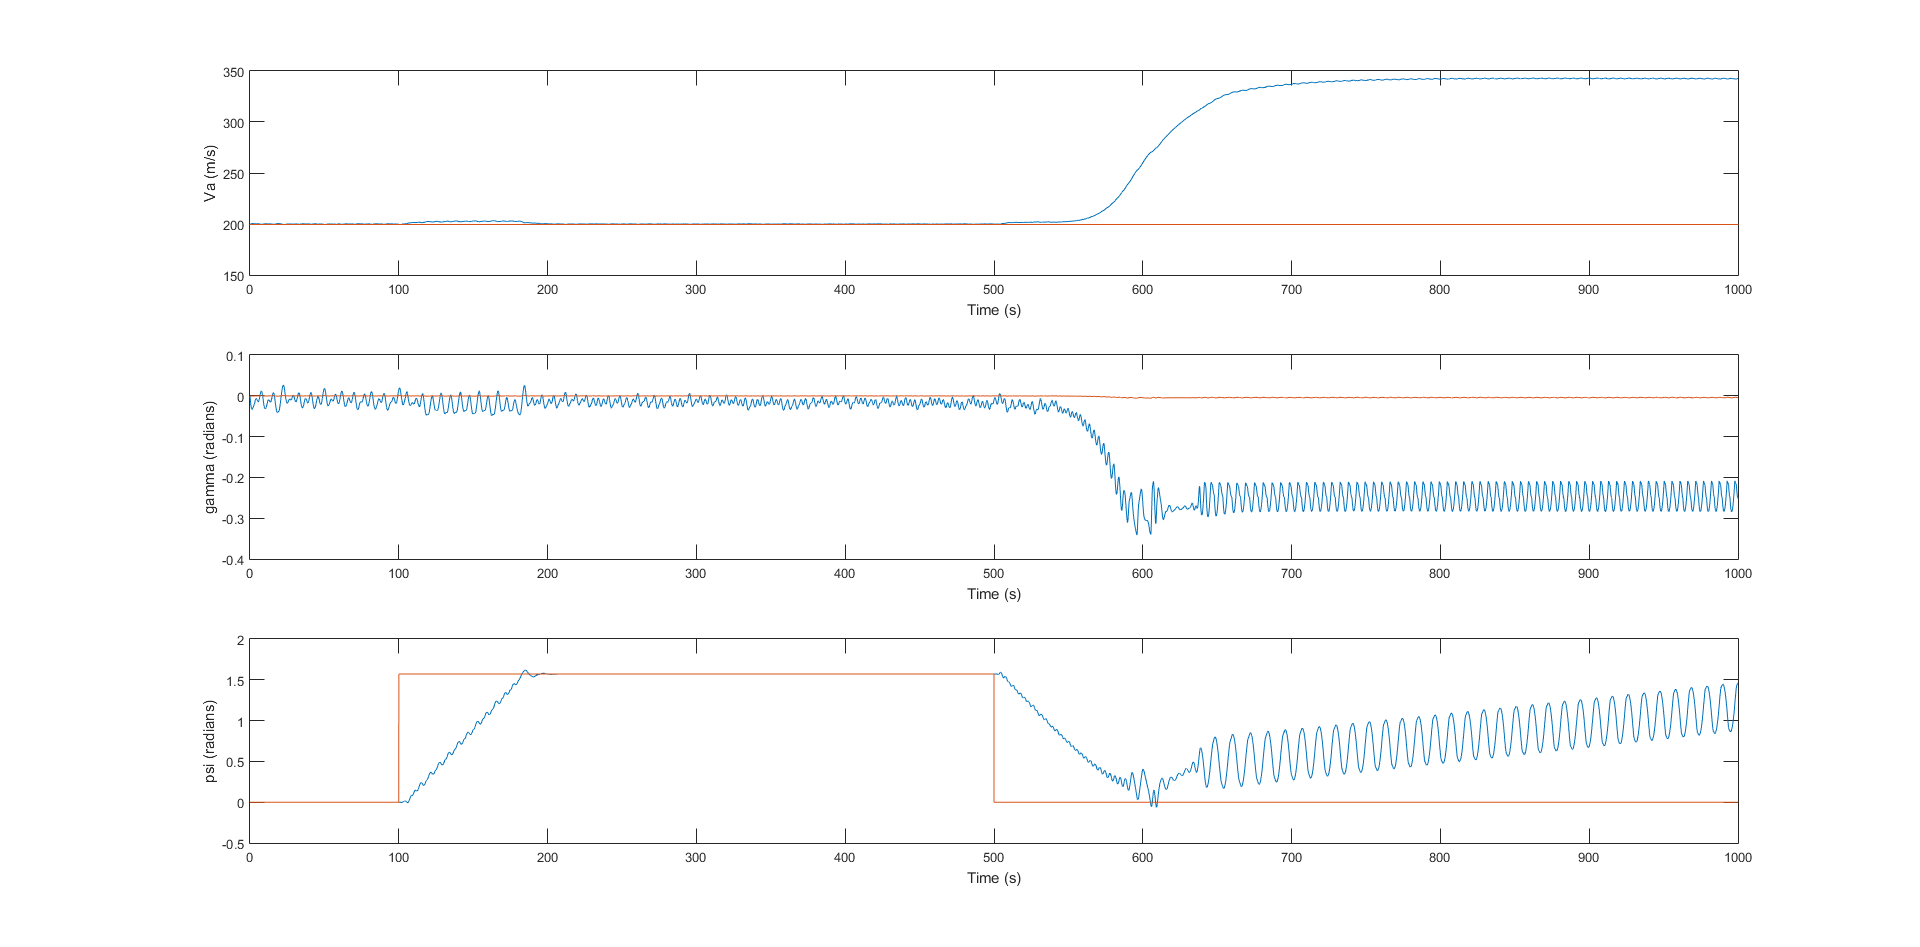
\includegraphics[width=1.1\textwidth]{Figures/Results/ref_zeta_005.png}
\caption[Reference tracking for $\zeta=0.05$]{$V_a$, $\gamma$ and $\psi$ for measured and desired values for $\zeta=0.05$}
\label{fig:ref_zeta_005}
\end{figure}

\subsection{Neural Network Correction}
The first adaptive capability of this method that will be described is the compensation of inversion error due to an incorrect estimation of the plane's inertia. Taking the previous example of \ref{fig:ref_zeta_005}, it can be observed that the aircraft becomes unstable at $t=600s$, leading to a significant increase of airspeed from the desired $200ms^{-1}$ to $350ms^{-1}$. The heading of the aircraft also becomes uncontrollable, oscillating and slowly increasing. 

This is due to the $\Delta$ component of equation \ref{eq:inversion_error}. At each time step the online Neural Network will converge to this value, compensating this error and therefore decreasing the reference following errors and preventing the aircraft from becoming unstable. Using the same conditions as used to obtain \ref{fig:ref_zeta_005} comes fig. \ref{fig:ref_zeta_005_NN}

\begin{figure}[H]
\centering
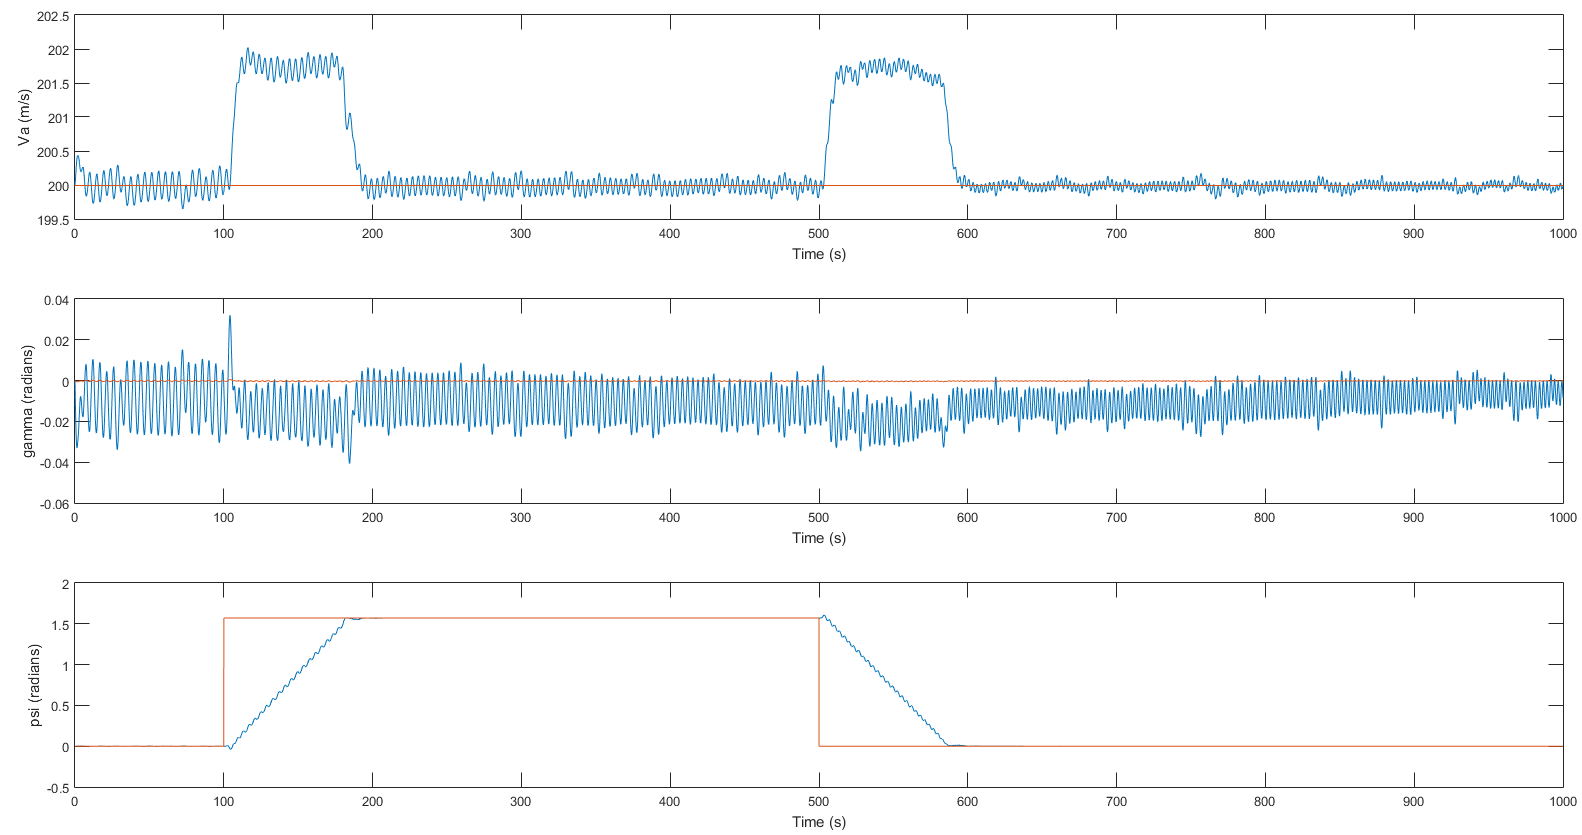
\includegraphics[width=1.1\textwidth]{Figures/Results/ref_zeta_005_NN.png}
\caption[Reference tracking for $\zeta=0.05$ with NN correction]{$V_a$, $\gamma$ and $\psi$ for measured and desired values for $\zeta=0.05$ with NN correction}
\label{fig:ref_zeta_005_NN}
\end{figure}

This first result shows for the adaptive control some improvements, mainly when comparing after $t=600s$. Comparing the airspeed, the value $V_a$ remains close to the desired value of $200ms^{-1}$ without reaching greater values, as observed previously. Regarding the yaw, besides an expected delay reaching the desired values, the system follows the reference with little to no error, this time without becoming unstable after $t=600s$. 

In order to more accurately visualise the influence of $\zeta$ on the NLI controller for this same case, several simulations were made for values of $\zeta$ from $0$ to $1$. For each simulation the mean error was computed, in order to obtain a plot of these errors for each of the three references. From figure  \ref{fig:xi_mean_error} can be concluded that the error becomes considerable $\zeta<0.05$ for a controller without neural network compensation. For a compensated adaptive controller however, it is noticeable that errors only become considerable at $\zeta<0.02$.


\begin{figure}[h]
\centering
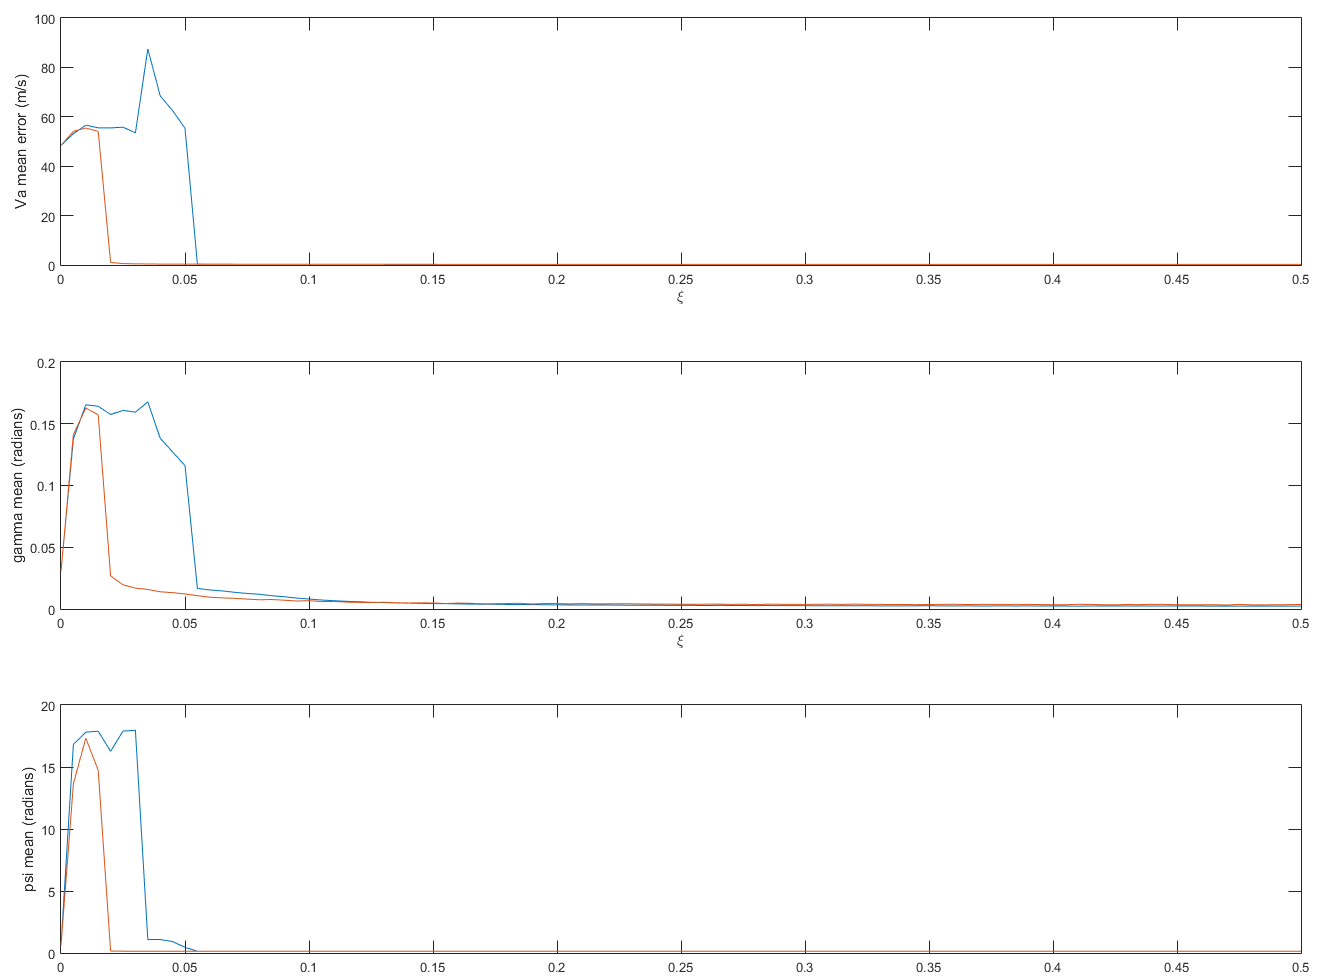
\includegraphics[width=1.1\textwidth]{Figures/Results/mean_error_xi.png}
\caption[Mean errors for $V_a$, $\gamma$ and $psi$]{Mean errors for $V_a$, $\gamma$ and $psi$ for $\zeta=[0,0.5]$ with neural network compensation (orange) and without compensation (blue)}
\label{fig:xi_mean_error}
\end{figure}

Studying the mean errors for $\zeta>1$, such an error represents a different situation. In this case, the estimated inertia of the aircraft is smaller than its real value. This can be caused by fuel consumption or, for the case of military aircraft, cargo release during flight. Reproducing the simulations from figure \ref{fig:xi_mean_error}, with $\zeta=[1,10]$, the results are obtained as in figure \ref{fig:xi_mean_error_big}.

\begin{figure}[H]
\centering
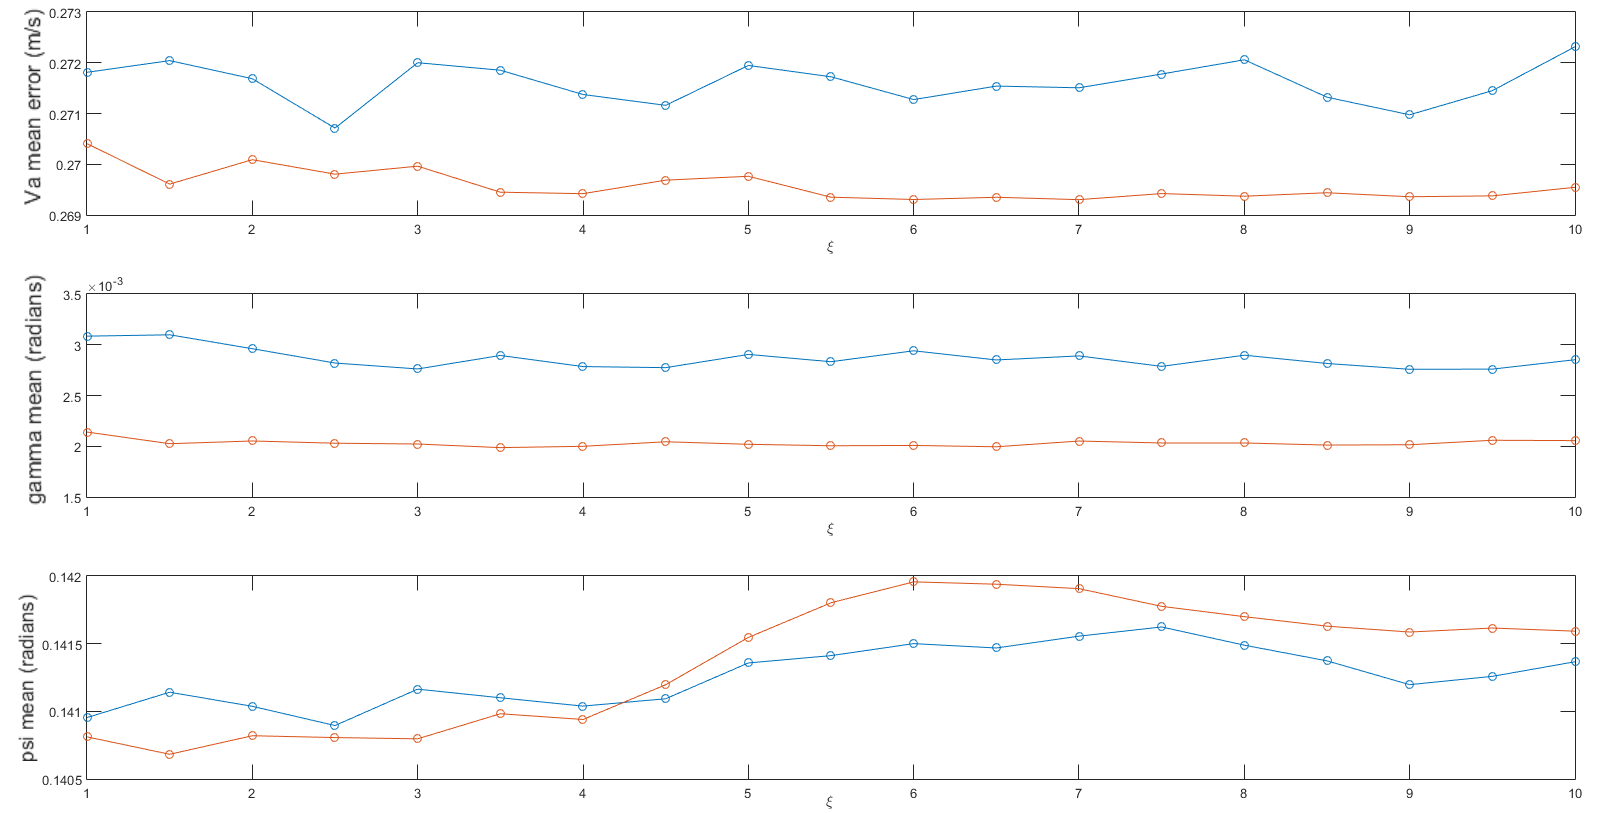
\includegraphics[width=1.1\textwidth]{Figures/Results/mean_error_xi_big.png}
\caption[Mean errors for $V_a$, $\gamma$ and $psi$ for larger values of $\zeta$ ]{Mean errors for $V_a$, $\gamma$ and $psi$ for $\zeta=[1,10]$ with neural network compensation (orange) and without compensation (blue)}
\label{fig:xi_mean_error_big}
\end{figure}

Although the errors showed in figure \ref{fig:xi_mean_error_big} are small and almost neglectable for these values of $\zeta$, these results still show, for $\gamma$ and $V_a$, the NN is capable of reducing the mean error when compared to the non corrected controller. This one however is able to perform correctly with a small tracking error for larger values of $\zeta$.

Although the network does seem to provide an adaptive component to the controller, note that it can only do so if the aircraft is operating within its limitation and the physically possible. Giving, for example, very low $V_a$ commands that wont provide the necessary lift for the aircraft will result, as would be expected, in an uncontrollable aircraft. Indeed, as seen in table \ref{tab:cruise_cond}, a $V_a$ value close to $200ms^{-1}$ is needed to maintain the necessary lift. The same also happens if, by simulating actuation failures, the values of $C_{\delta_{ail}}, C_{\delta_{ele}}, C_{\delta_{rud}}$ are too excessively reduced, or if the system is subjected to extreme icing and wind conditions that would render the aircraft unflyable. For these results the conditions were chosen so that while these would increase the command error of the baseline controller, the airplane would still be flyable allowing the network to improve its controllability and reduce this error.

The designed controller, as detailed in section \ref{section:control_implement}, includes a linear controller for the system linearised by the nonlinear inversion, more precisely a PD controller for the plane's fast dynamics. A poorly tuned controller however will lead to an undesired behaviour. Using once again the condition used so far (see figure \ref{fig:ref_zeta_05}, with a perfect inertia estimation $\zeta = 1$ from a reduced controller, compared to the same controller corrected by the NN, comes that:

\begin{figure}[h]
\centering
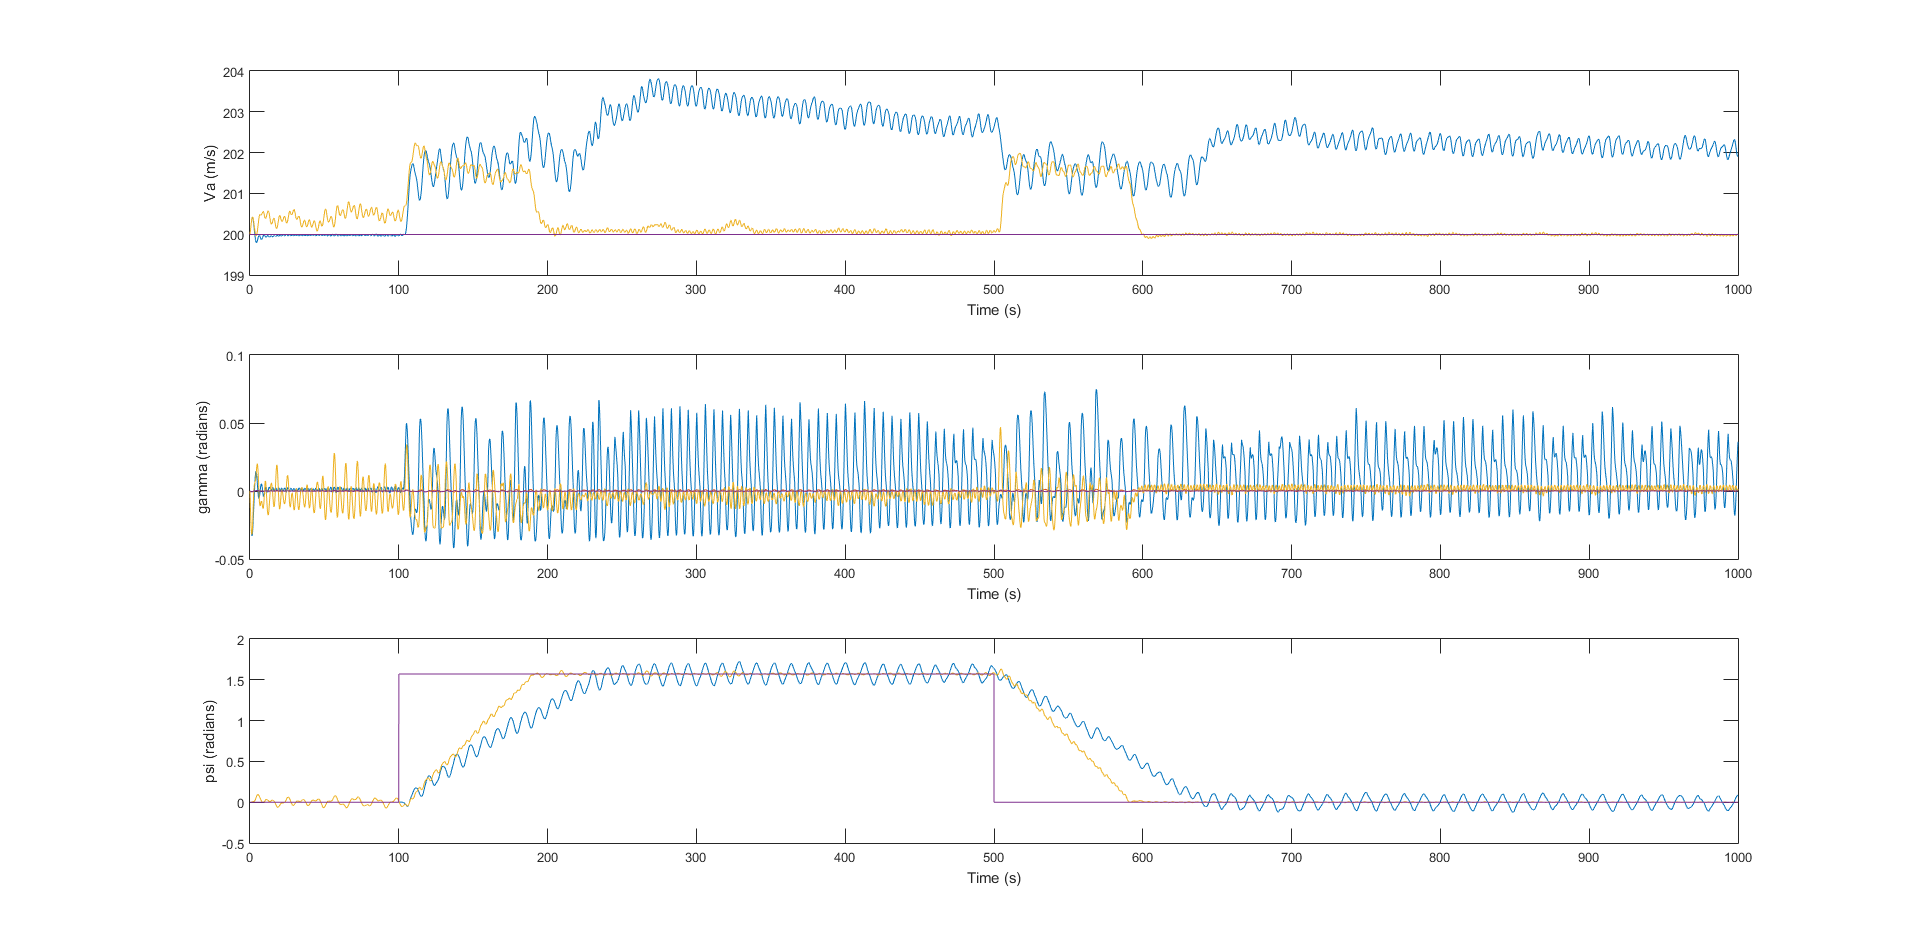
\includegraphics[width=1.1\textwidth]{Figures/Results/ref_bad_control.png}
\caption[Poorly tuned controller comparison]{$V_a$, $\gamma$ and $\psi$ for measured and desired values. In purple can be seen the three references, in blue can be seen the measured values where in equation \ref{eq:linear_controller} $K_D=0$ and $K_P = [1,1,1]^T$. In yellow the same controller is used, while applying NN adaptive corrections}
\label{fig:ref_bad_control}
\end{figure}

The first observation that can be taken from figure \ref{fig:ref_bad_control} is that the difference the purple and yellow graphs is considerably smaller than that of the blue graph, particularly noticeable in the first $V_a$ plot. In the two last ones oscillations around the desired value are reduced, as is the yaw convergence time for the NN adaptive controller by $30s$.
It is also curious to observe the oscillations of yellow neural network adapted plot decrease with time. This is explained as the weights of the network do not converge instantly to their optimal values.

\section{System Failures}
\label{section:results/system_failures}

\subsection{Baseline Feedback Linearisation Controller}
One other cause for inversion errors that can have a great impact on flight trajectory are system failures. This subsection will focus on methods to simulate these failures and observe the behaviour of the airplane trajectory for these cases. The reference trajectory that will be used will be the same as used previously. The first failure to be simulated will be a control surfaces failure, that will lead to reduced controllability of the aircraft. In this work this was replicated in a simulated environment by reducing each moment coefficients for the elevator, aileron and rudder, namely $C_{\delta_{ele}}$, $C_{\delta_{ail}}$ and $C_{\delta_{rud}}$.

By setting each of these coefficients to 20\% of their initial values, the effect of the errors in followed trajectory become visible in figure \ref{fig:reduced_act}. This figure shows that the reduced controllability results in a $20km$ difference to that of the undisturbed system. This sets the second goal for the performance of the neural network, to reduce this error as much as possible. This is a preliminary analysis, as actuator failures can a much bigger impact on the aircraft flight and can even render it uncontrollable. For this simulation however, the goal was to simulate failures that would only reduce the controllability of the aircraft, to then use the NN to improve its behaviour. 

\begin{figure}[H]
\centering
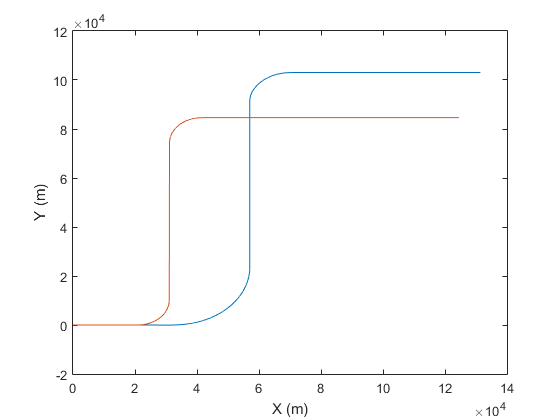
\includegraphics[width=0.8\textwidth]{Figures/Results/reduced_act.png}
\caption[Trajectory with reduced actuation]{Trajectory with 20\% reduced actuation (blue) and trajectory without failures (red)}
\label{fig:reduced_act}
\end{figure}

Studying as previously the values of $V_a$, $\gamma$ and $\psi$ for the case of actuator failures, the following results are obtained 

\begin{figure}[h]
\centering
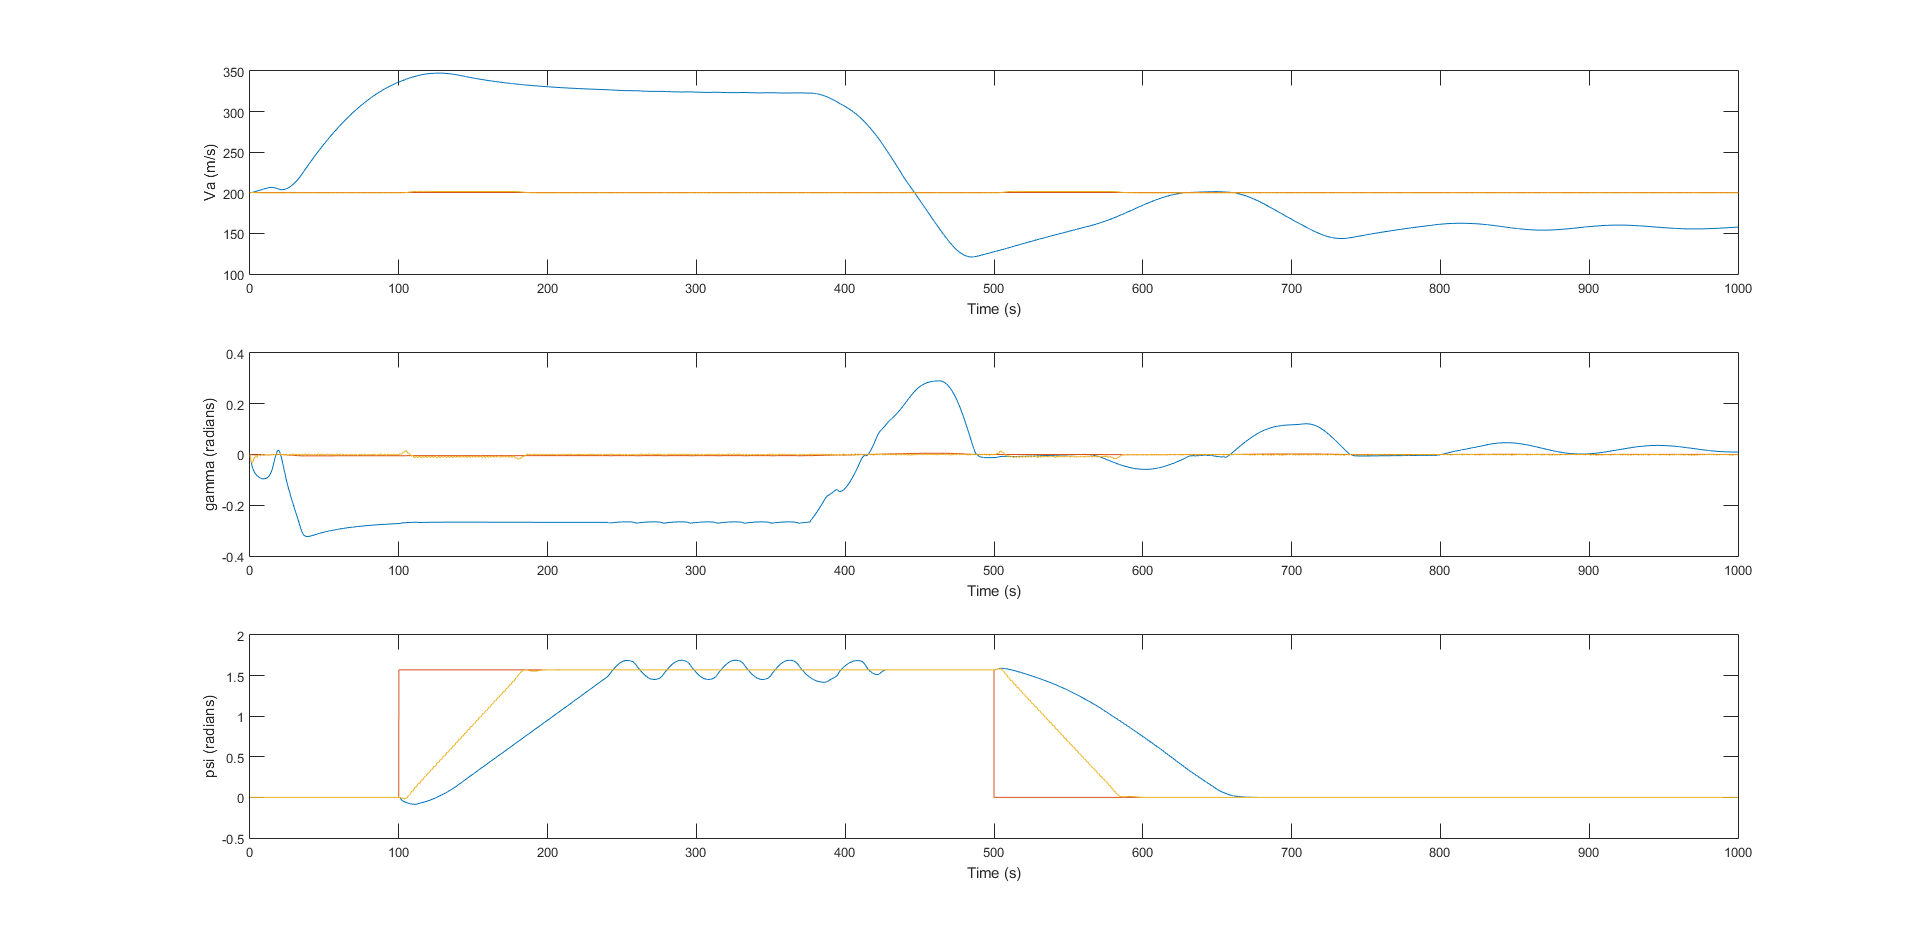
\includegraphics[width=1.1\textwidth]{Figures/Results/ref_act_failure.png}
\caption[$V_a$, $\gamma$ and $\psi$ measured and desired values on actuation failure]{$V_a$, $\gamma$ and $\psi$ desired  values (orange), measured without actuator failures (yellow) and with reduced actuation (blue)}
\label{fig:ref_act_fail}
\end{figure}

From figure \ref{fig:ref_act_fail} the first conclusion that can be drawn is that the tracking error for the simulation with actuator failures is considerably greater than the simulation without failures for $V_a$ and $\gamma$. $V_a$ increases up to $150ms{-1}$ above its reference values, whereas $\gamma$ initially decreases down to $-14^o$. Both of these values are unrealistic for such a commercial aircraft and are caused by the reduced control surface moments. The effect of these reduced moments is also noticeable for $\psi$, that in case of actuator failures takes twice as long, up to $160s$ to reach its reference value, up from $90s$ without these failures.

One second type of flight perturbation that will be included in this subsection is the effects of icing conditions in aircraft flight. According to the FAA guide to flight in icing conditions, ice contamination of an airfoil has an important influence on both the Lift and Drag curves \cite{icing_cond}. Ways to simulate these perturbations in a modelled environment will be studied, and as for the other described disturbances an online neural network will be used to improve the control of the aircraft in such conditions. The main drawbacks that can be caused by icing are

\begin{itemize}
\item \textbf{Stall }As seen in figure \ref{fig:icing_lift}, ice contamination of the airfoil leads to a significant reduction in the value of the maximum $C_L$, causing the aircraft to reach stall conditions at a much lower angle of attack. Reducing speed (e.g for an approach) makes this effect more noticeable for the pilot. The usual reduction on $C_{L_{max}}$ is of 30\% \cite{icing_cond}.

\item \textbf{Drag }Drag will increase directly with the amount of ice accumulated on the wing, reaching usual values of 100\% of the initial drag coefficient.

\item \textbf{Roll }Icing on the main wings will also affect roll control. As the thickness of the wing decreases towards its tip, so increases its efficiency to collect ice, leading to a partial stall in the tip of the wings, according to the AOPA manual \cite{icing_aopa}.
\end{itemize}
\begin{figure}[H]
\centering
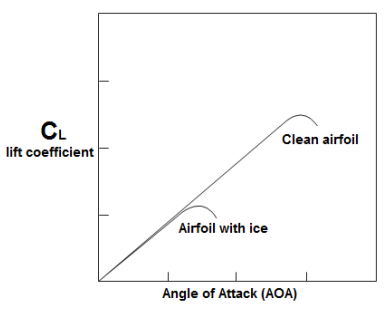
\includegraphics[width=0.5\textwidth]{Figures/Results/icing_lift.PNG}
\caption[Effects of icing on lift coefficient]{Effects of icing on lift coefficient \cite{icing_cond}}
\label{fig:icing_lift}
\end{figure}
\begin{figure}[H]
\centering
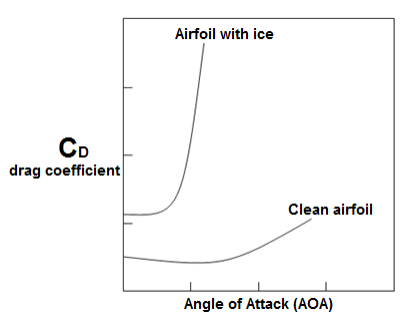
\includegraphics[width=0.5\textwidth]{Figures/Results/icing_drag.PNG}
\caption[Effects of icing on drag coefficient]{Effects of icing on drag coefficient \cite{icing_cond}}
\label{fig:icing_drag}
\end{figure}

Following these indications to simulate heavy icing condition, the lift coefficient $C_{L_{max}}$ was reduced by 30\%, and the stall angle reduced from $15^o$ (see figure \ref{fig:cl_alpha}) resulting in figure \ref{fig:cl_icing}. The value of the drag coefficient was also augmented by 200\% from equation \ref{eq:cd_cl}. Finally, in order to simulate roll control limitations, the value of $C_{\delta_{ail}}$ was reduced by 30\%. These values were chosen in order to deteriorate the control of the aircraft, while allowing for the possibility of reference following without reaching actuator saturation (for both control surface deflections and thrust). 

For this case a sinusoidal yaw reference was given of $\psi^d= \dfrac{\pi}{4} \sin (1.1459t)\text{ rad}$, $t$ being the simulation time. A sinusoidal reference was used to make the effects of simulated icing more noticeable, and the same references of $V_a^d=200ms^{-1}$ and $\gamma^d=0\text{ rad}$ as previously were used. For this case, the results obtained were as follows

\begin{figure}[H]
\centering
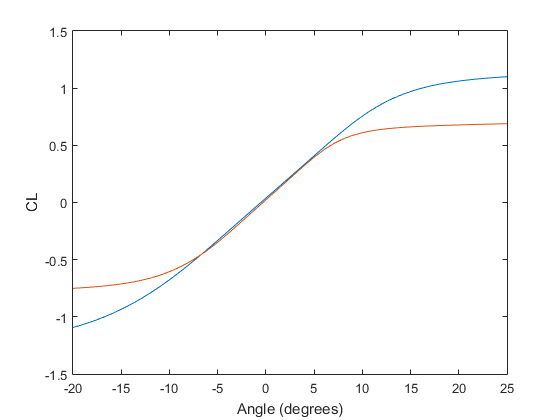
\includegraphics[width=1\textwidth]{Figures/Results/cl_icing.PNG}
\caption[Lift coefficient simulation in icing conditions]{Lift coefficient simulation in icing conditions (orange) and in normal conditions (blue)}
\label{fig:cl_icing}
\end{figure}

\begin{figure}[H]
\centering
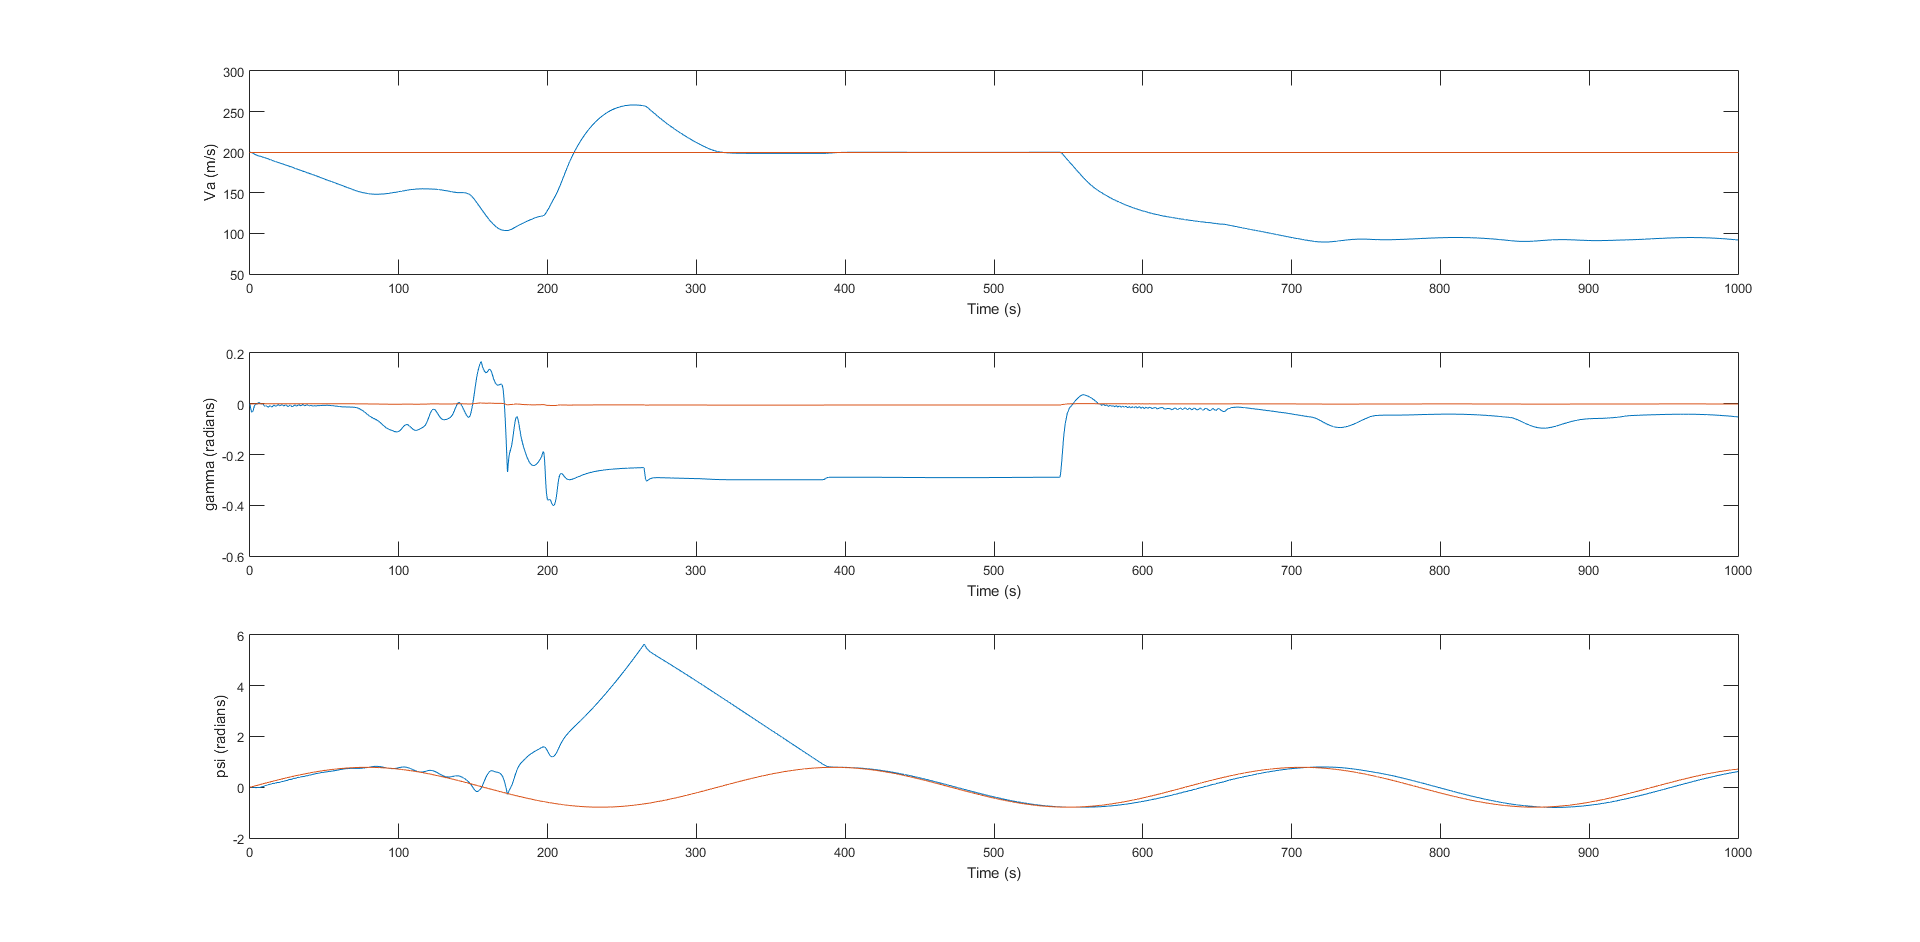
\includegraphics[width=1.1\textwidth]{Figures/Results/ref_icing.PNG}
\caption[Reference following in icing conditions]{$V_a$, $\gamma$ and $\psi$ for measured and desired values in icing conditions}
\label{fig:ref_icing}
\end{figure}

From figure \ref{fig:ref_icing}, the system in such high drag conditions can be considered marginally stable, as it easily increases the error to either of the three commanded inputs to significantly high values. For the case of the flight path angle, the aircraft even reaches under $-20º$ at $t=600s$, a completely unrealistic value for a normal cruise flight. The impact of the increased drag in noticeable in the reduced speed in the simulation, going under $100ms^{-1}$ for the desired $V_a^d=200ms^{-1}$. The reduced roll capabilities and lift also cause errors and oscillations in heading and flight path angle following.


These perturbations change the expected behaviour of the aircraft, causing the feedback linearisation control law to perform poorly. In the next section of this work the results of the online neural network will be shown, demonstrating its ability to increase the stability of the aircraft in situations of strong perturbations, or even in cases of a poorly designed linear or feedback linearisation controller. Note however that the conditions used here to induce the aircraft into unstable or marginally stable conditions mimic extreme perturbations, and the described controller can be said to perform well in cases when little to none of these perturbations are present.

\subsection{Neural Network Correction}

The next objective will be to observe if the designed controller is capable of adapting to system failures. Simulation of these failures was described in the previous subsection, where actuator failures and icing conditions were tested. 

\subsubsection{Actuator failure}

In the same conditions as previously, the aerodynamic coefficients of the control surfaces were reduced to 20\% of their initial values. Applying the adaptive correction through the online neural network, the following trajectories were obtained

\begin{figure}[H]
\centering
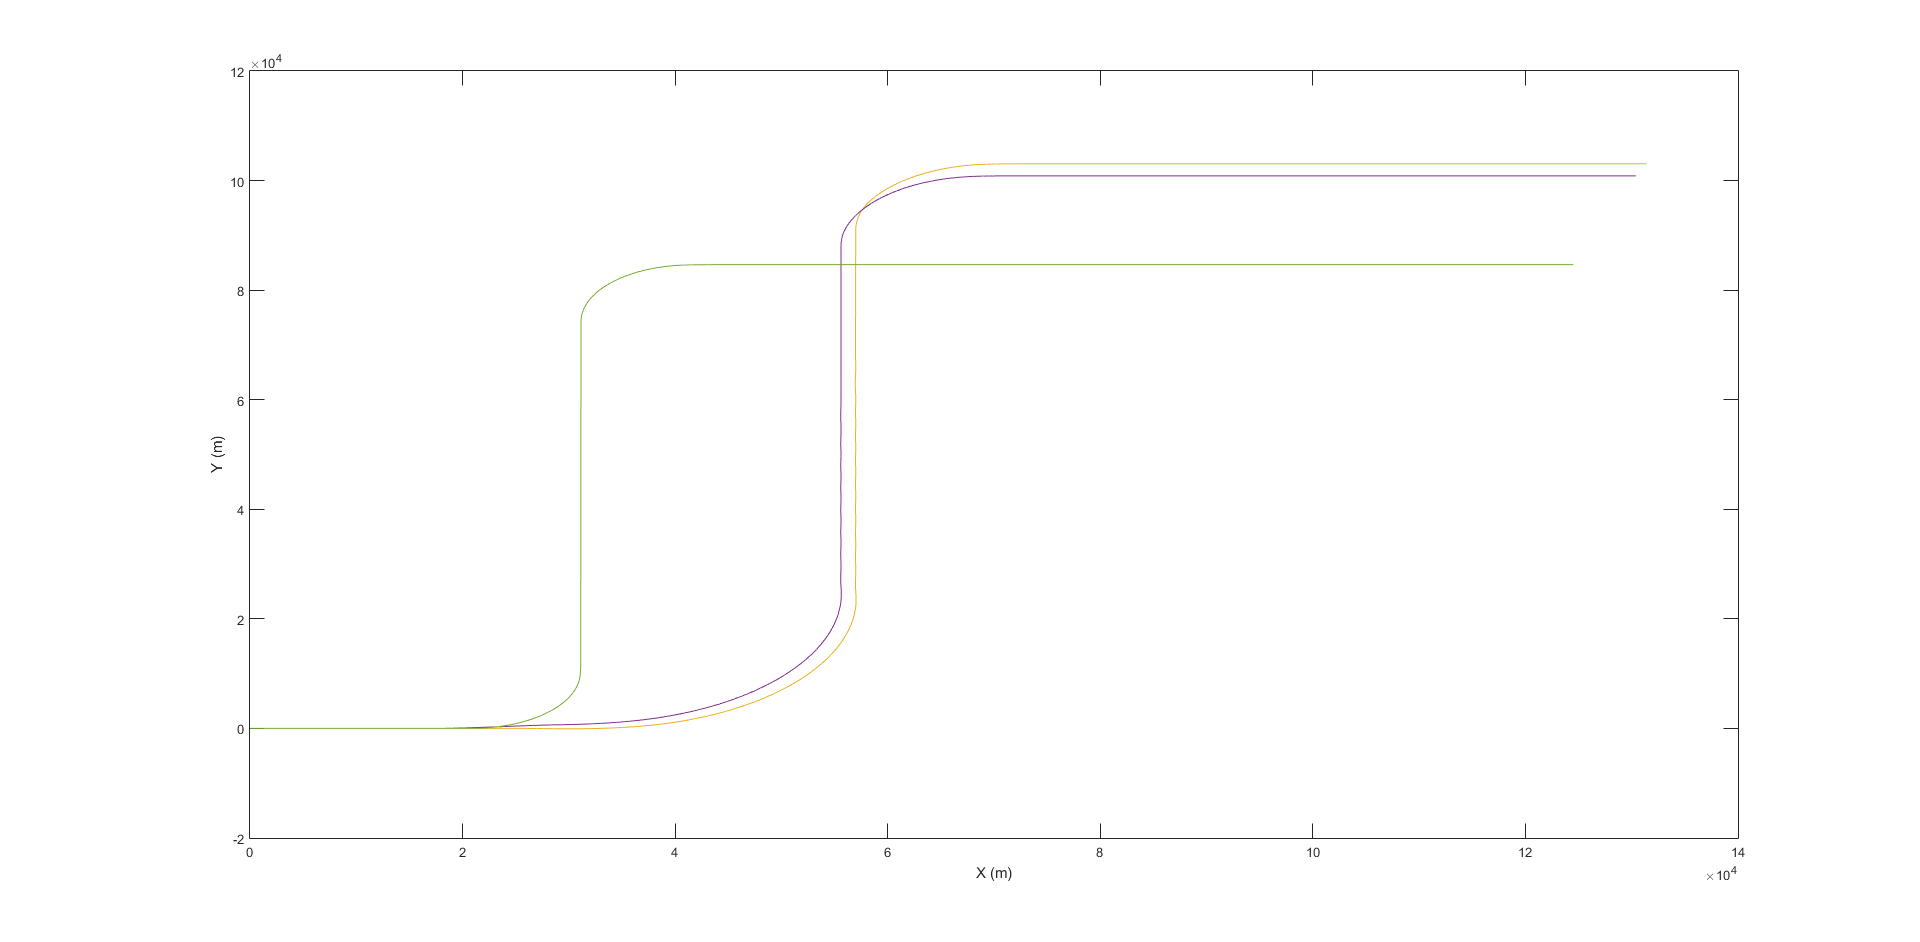
\includegraphics[width=\textwidth]{Figures/Results/reduced_act_NN.png}
\caption[Trajectory with reduced actuation corrected with NN correction]{Trajectory with 20\% reduced actuation (yellow) and trajectory without failures (green). The corrected trajectory by the NN can be seen in purple}
\label{fig:reduced_act_NN}
\end{figure}

The first observation that can be drawn from figure \ref{fig:reduced_act_NN} is that such an actuator failure severely reduces the controllability of the aircraft. 

The main consequence for this case will be, as could be expected, an increase in the convergence time to the desired heading. Note that the desired trajectory is not followed as this correction is only applied to the fast dynamics, and a guidance control law is not yet implemented. Comparing the two cases where the failures were implemented however, it can be observed that system corrected by the neural network converged to the desired heading slightly faster, resulting in a $2000m$ reduction in distance when comparing the non corrected control trajectory.

\begin{figure}[H]
\centering
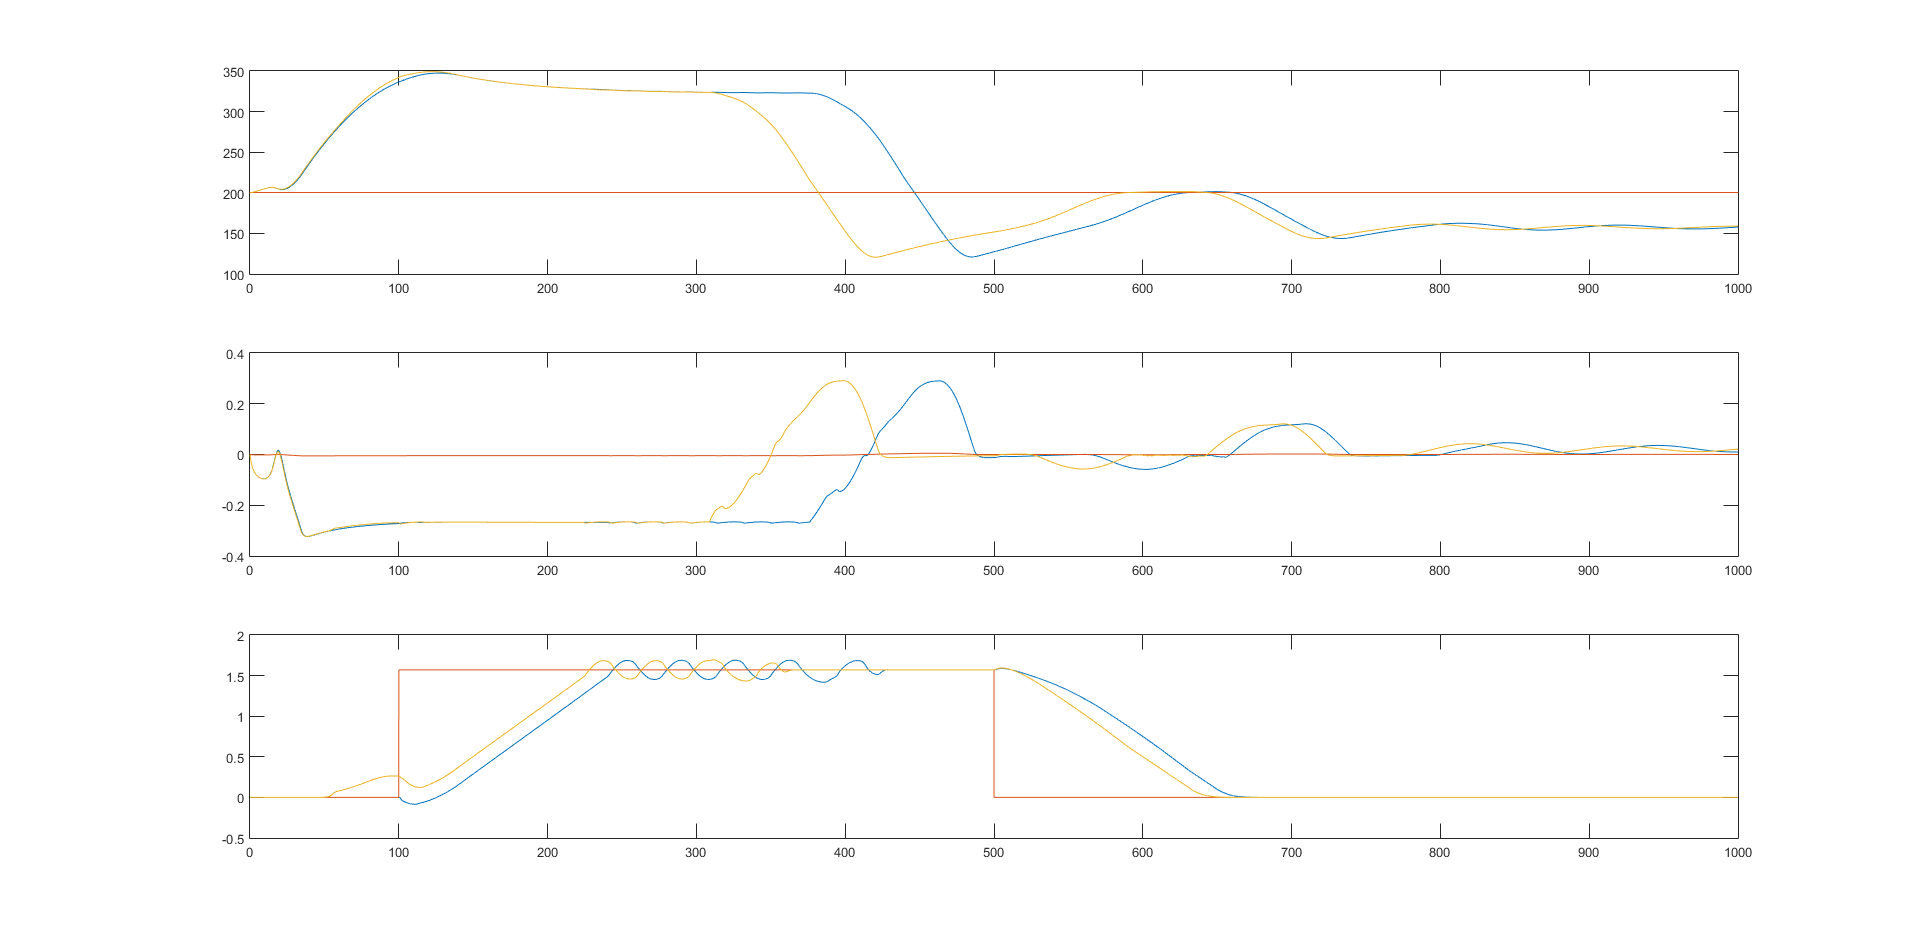
\includegraphics[width=1.1\textwidth]{Figures/Results/ref_act_failure_NN.png}
\caption[$V_a$, $\gamma$ and $\psi$ measured and desired values on actuation failure with NN correction]{$V_a$, $\gamma$ and $\psi$ desired  values (red), measured with actuator failures and NN correction (yellow) and without NN correction (blue)}
\label{fig:ref_act_fail_NN}
\end{figure}

Observing this system with the NN corrections, the error with such failures is still just as large as without NN correction, although the network seems to have a lead to the non corrected simulation, causing it to reach stable values faster and, for the case of $\psi$, to have a shorter delay reaching the desired heading.  

\subsubsection{Icing conditions}

Once again retaking the example from figure \ref{fig:ref_icing}, in the same icing conditions, the online network correction was applied, resulting in the following results

\begin{figure}[H]
\centering
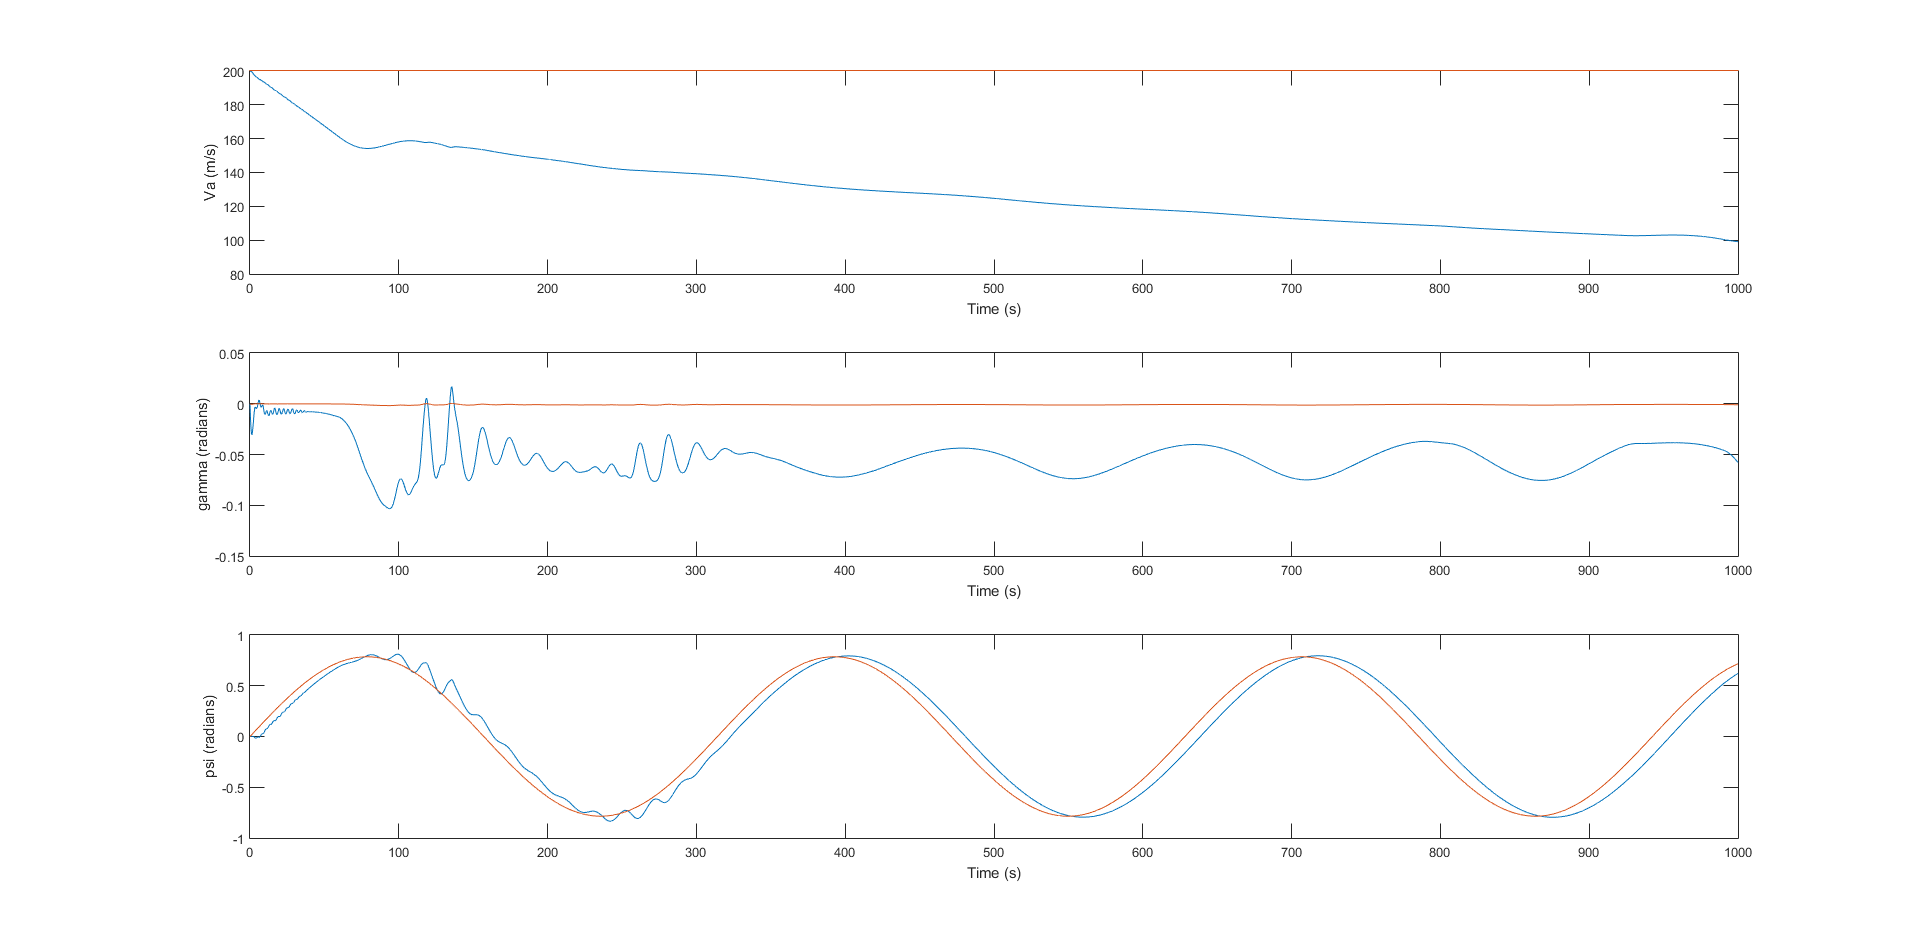
\includegraphics[width=1.1\textwidth]{Figures/Results/ref_icing_NN.PNG}
\caption[Reference following in icing conditions with NN correction]{$V_a$, $\gamma$ and $\psi$ for measured and desired values in icing conditions, with NN correction}
\label{fig:ref_icing_NN}
\end{figure}

Again, these are conditions that have a negative impact on the controllability of the aircraft: the increase of 200\% of the value of $C_D$ causes a decrease in the speed of the aircraft, rendering it unable to follow the desired speed of $200ms^{-1}$. Regarding the measured flight path angle $\gamma$, although  some oscillations are still present, error relative to the reference no longer goes up to $0.3\text{ rad}$, instead oscillating around $0.05\text{ rad}$ at a much lower frequency and amplitude. The most noticeable improvement however can be seen in the heading following: the aircraft follows the desired $\psi^d$ during the full simulation, with little to no oscillations around that value. It is also interesting to notice that in the first moments of the learning process, up to $t=300s$, oscillations around the desired heading value are greater than in later moments of the simulation. This is explained by the fact that the weights of the neural network have not yet converged to their optimal values at $t<300s$.


\section{Guidance Controller}
\label{section:results/guidance_control}

This final section will focus on the results of the implementation of the guidance controller described in equations \ref{eq:guidance_law}. From the work implemented and results obtained thus far, a NN adaptive controller can now be used to follow references of airspeed, heading and flight path angle. From the equations \ref{eq:guidance_law} position references can now be used to compute $V_a,\gamma, \psi$. Choosing a path to follow using these equations the following results were obtained, showing the aircraft is able to correctly follow a trajectory from a constant feed of way points over time.

\begin{figure}[h]
\centering
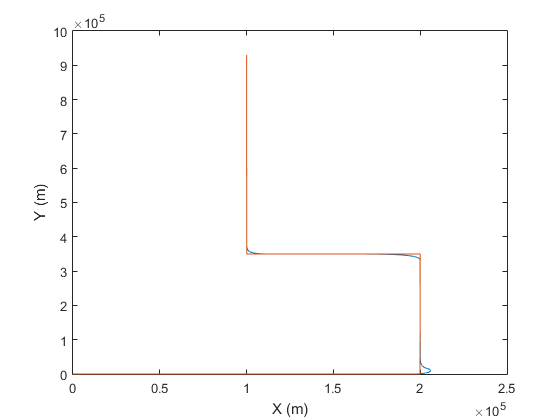
\includegraphics[width=1\textwidth]{Figures/Results/guidance.png}
\caption[Trajectory following with guidance controller]{Trajectory reference (orange) and obtained trajectory (blue)}
\label{fig:guidance}
\end{figure}



\begin{figure}[h]
\centering
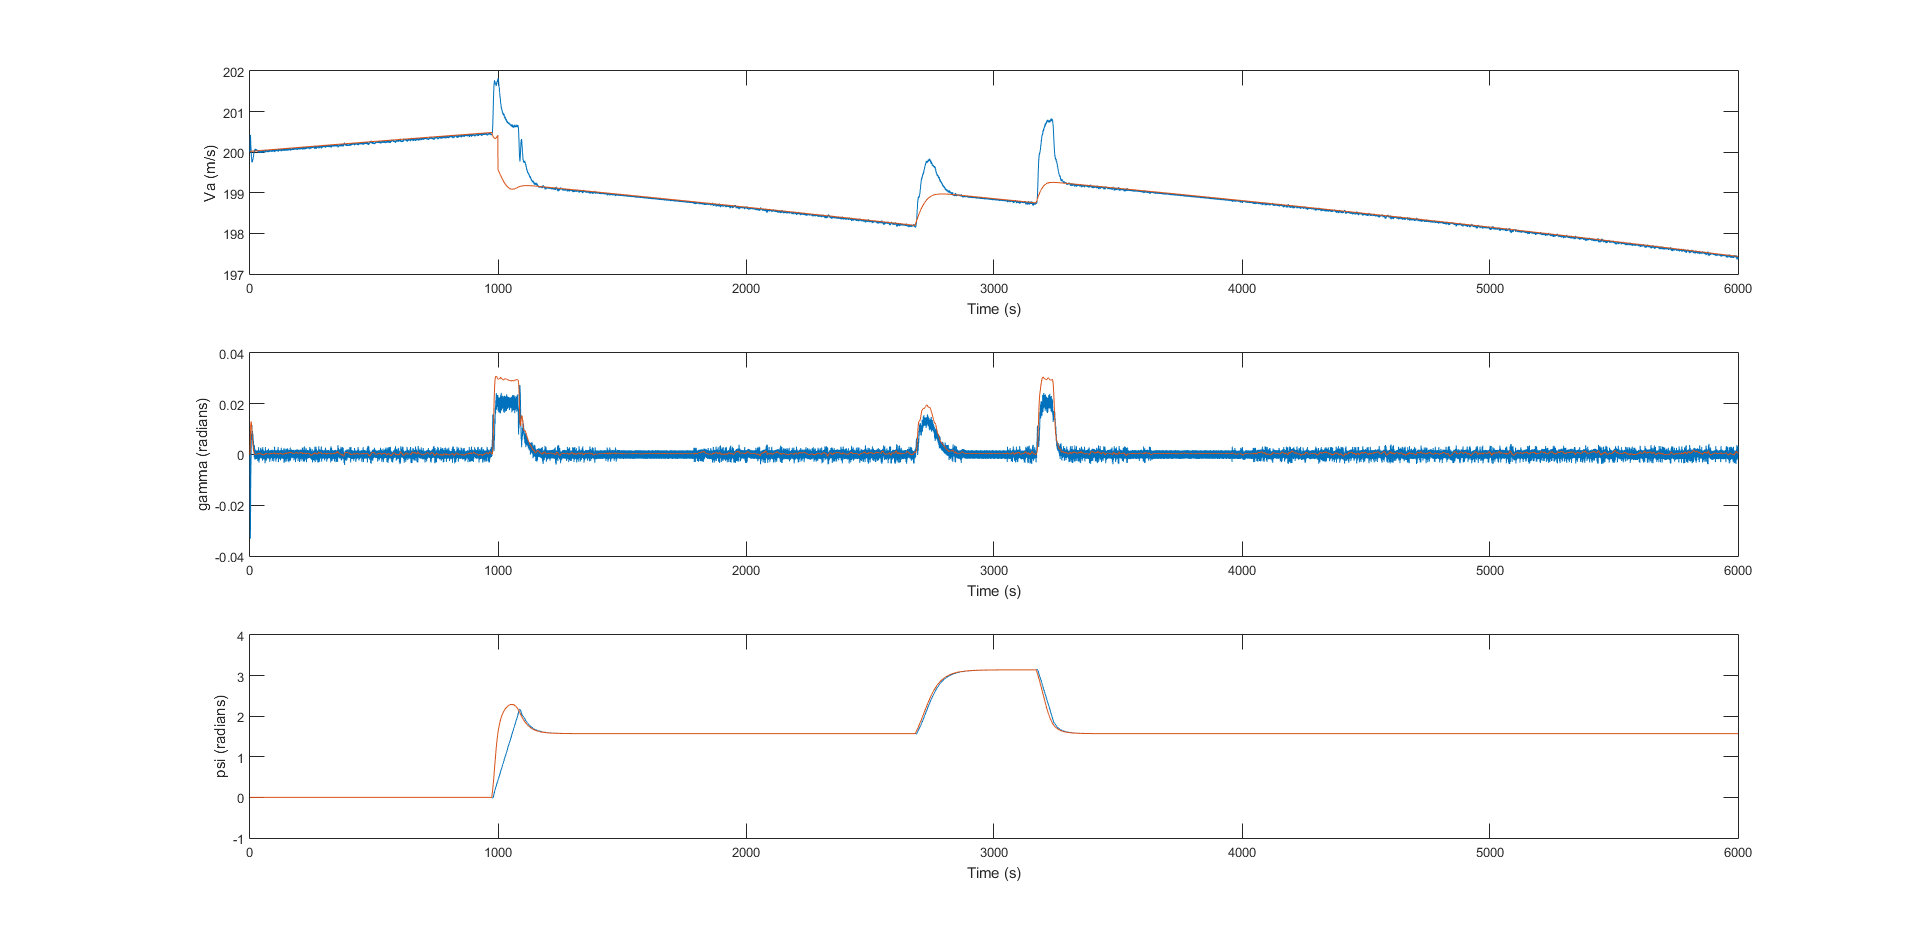
\includegraphics[width=1.15\textwidth]{Figures/Results/guidance_ref.png}
\caption[Reference following of $V_a$, $\gamma$ and $\psi$ from guidance controller]{$V_a$, $\gamma$ and $\psi$ for measured (blue) and desired values (orange) obtained from the guidance controller}
\label{fig:guidance_ref}
\end{figure}

\begin{figure}[h]
\centering
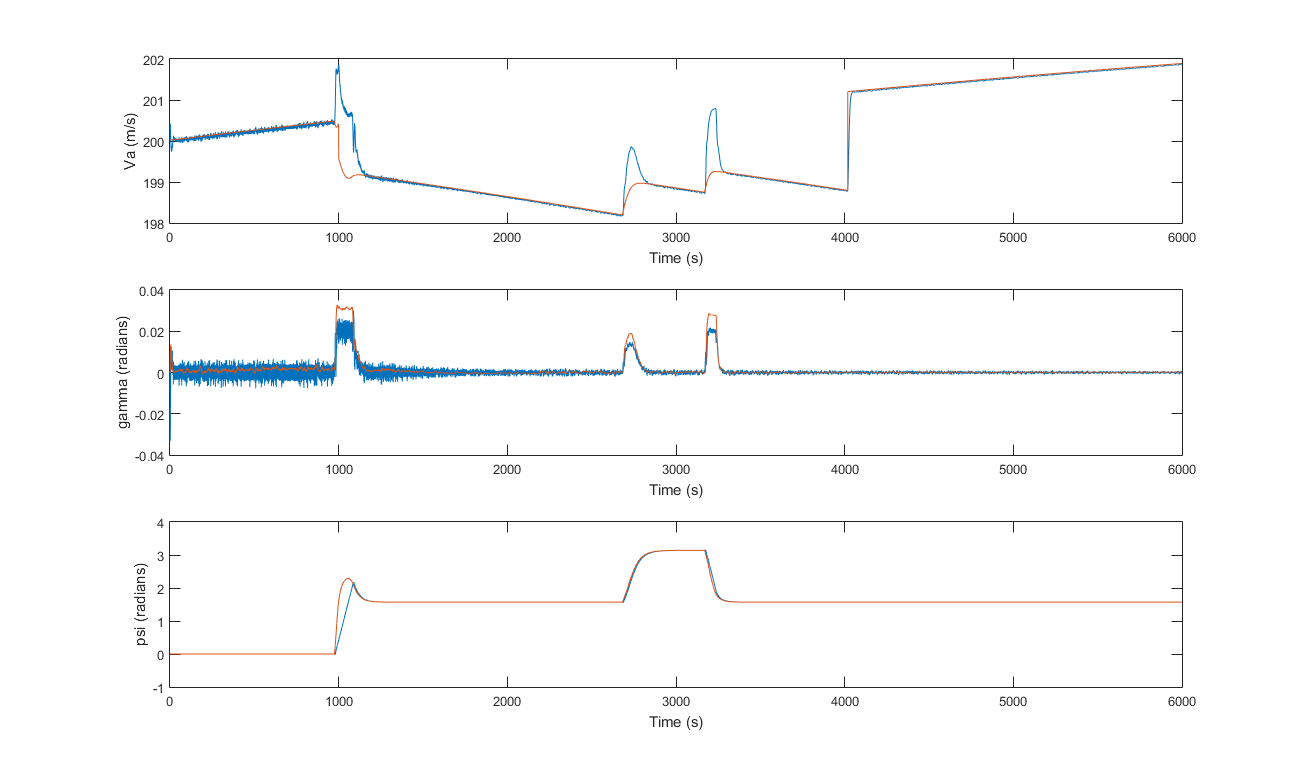
\includegraphics[width=1.15\textwidth]{Figures/Results/guidance_ref_NN.png}
\caption[Reference following of $V_a$, $\gamma$ and $\psi$ from guidance controller with NN correction]{$V_a$, $\gamma$ and $\psi$ for measured (blue) and desired values (orange) obtained from the guidance controller using NN correction}
\label{fig:guidance_ref_NN}
\end{figure}

Figure \ref{fig:guidance} shows the trajectory of the aircraft for a given trajectory, showing slight errors on sudden heading changes. Analysing figure \ref{fig:guidance_ref}, for a non corrected system, although a small overshoot in airspeed following, the three variable otherwise follow their references with minimal error. The $\gamma$ graph however shows that this variable oscillates around $0$ rad.

Comparing these results with the NN corrected controller however, although no disturbance was added to the simulation, the flight path angle oscillations are greatly reduced. It is also interesting to notice that while the network is still converging its weights to reach their optimal values for the first $1000s$, these oscillations are greater than in the $4000s$.